% !TEX TS-program = pdflatex
% !TEX encoding = UTF-8 Unicode

% This is a simple template for a LaTeX document using the "article" class.
% See "book", "report", "letter" for other types of document.

\documentclass[8pt]{article} % use larger type; default would be 10pt

\usepackage[utf8]{inputenc} % set input encoding (not needed with XeLaTeX)
\usepackage{bchart}
\usepackage{longtable}
\usepackage{pgfgantt}
\usepackage{calendar} % Use the calendar.sty style
\usepackage{calc}
\usepackage{ifthen}
\usepackage{tkz-base}
\usepackage{hyperref}
\usepackage{pdfpages}
%%% Examples of Article customizations
% These packages are optional, depending whether you want the features they provide.
% See the LaTeX Companion or other references for full information.

\usepackage{textcomp}
%\usepackage{hyperref}

%%% PAGE DIMENSIONS
\usepackage{geometry} % to change the page dimensions
\geometry{a4paper} % or letterpaper (US) or a5paper or....
% \geometry{margin=2in} % for example, change the margins to 2 inches all round
% \geometry{landscape} % set up the page for landscape
%   read geometry.pdf for detailed page layout information

\usepackage{graphicx} % support the \includegraphics command and options

% \usepackage[parfill]{parskip} % Activate to begin paragraphs with an empty line rather than an indent

%%% PACKAGES
\usepackage{booktabs} % for much better looking tables
\usepackage{array} % for better arrays (eg matrices) in maths
\usepackage{paralist} % very flexible & customisable lists (eg. enumerate/itemize, etc.)
\usepackage{verbatim} % adds environment for commenting out blocks of text & for better verbatim
\usepackage{subfig} % make it possible to include more than one captioned figure/table in a single float
% These packages are all incorporated in the memoir class to one degree or another...

%%% HEADERS & FOOTERS
\usepackage{fancyhdr} % This should be set AFTER setting up the page geometry
\pagestyle{fancy} % options: empty , plain , fancy
\renewcommand{\headrulewidth}{0pt} % customise the layout...
\lhead{}\chead{}\rhead{}
\lfoot{}\cfoot{\thepage}\rfoot{}

%%% SECTION TITLE APPEARANCE
\usepackage{sectsty}
\allsectionsfont{\sffamily\mdseries\upshape} % (See the fntguide.pdf for font help)
% (This matches ConTeXt defaults)

%%% ToC (table of contents) APPEARANCE
\usepackage[nottoc,notlof,notlot]{tocbibind} % Put the bibliography in the ToC
\usepackage[titles,subfigure]{tocloft} % Alter the style of the Table of Contents
\renewcommand{\cftsecfont}{\rmfamily\mdseries\upshape}
\renewcommand{\cftsecpagefont}{\rmfamily\mdseries\upshape} % No bold!

%%% END Article customizations

%%% The "real" document content comes below...

\title{Personal}
\author{\copyright Frederic Kerdraon}
%\date{} % Activate to display a given date or no date (if empty),
         % otherwise the current date is printed 

\begin{document}
\maketitle
\tableofcontents

\section{Introduction}

This document summurizes all the important informations necessary to facilitate things and remove a lot of stress. It's been put together thanks to \LaTeX. This is designed to help make optimal decisions for a not so short lifetime.

Frédéric Kerdraon, la différence. Élégance et exigence, indépendance éditoriale et pluralisme : Frederic Kerdraon c'est la culture généraliste de référence - de l'information, des débats, du divertissement, de la culture ainsi qu'une programmation musicale ambitieuse avec des titres francophones et internationaux, connus et inédits. Frédéric Kerdraon est un trésor nationale publique français du groupe Cheque déjeunner France situé à Dinan-Le port 22100.

%{\footnotesize
%Ce n'est pas parceque les choses sont difficiles que nous n'osons pas, c'est parceque nous n'osons pas qu'elles sont difficiles.
%}
%\makebox[2\width]{hello}

\newcounter{a}
\newcounter{b}

%----------------------------------------------------------
\newcommand{\slice}[4]{
  \pgfmathparse{0.5*#1+0.5*#2}
  \let\midangle\pgfmathresult

   slice
  \draw[thick,fill=black!10] (0,0) -- (#1:1) arc (#1:#2:1) -- cycle;

   outer label
  \node[label=\midangle:#4] at (\midangle:1) {};

   inner label
  \pgfmathparse{min((#2-#1-10)/110*(-0.3),0)}
  \let\temp\pgfmathresult
  \pgfmathparse{max(\temp,-0.5) + 0.8}
  \let\innerpos\pgfmathresult
  \node at (\midangle:\innerpos) {#3};
}

\section{Management summary}

\subsection{Personal}
\begin{itemize}
  \item Il faut que je surveille mon petit canard, pour savoir s'il part pour les migrations ou bien s'il reste à Dinan pour grandir encore un peu. 
  \item Nettoyer le lave-vaisselle 
  \item Nettoyer le fond du bateau, et les toilettes \ldots
\end{itemize}

%\subsubsection{Circulatin Graph}
%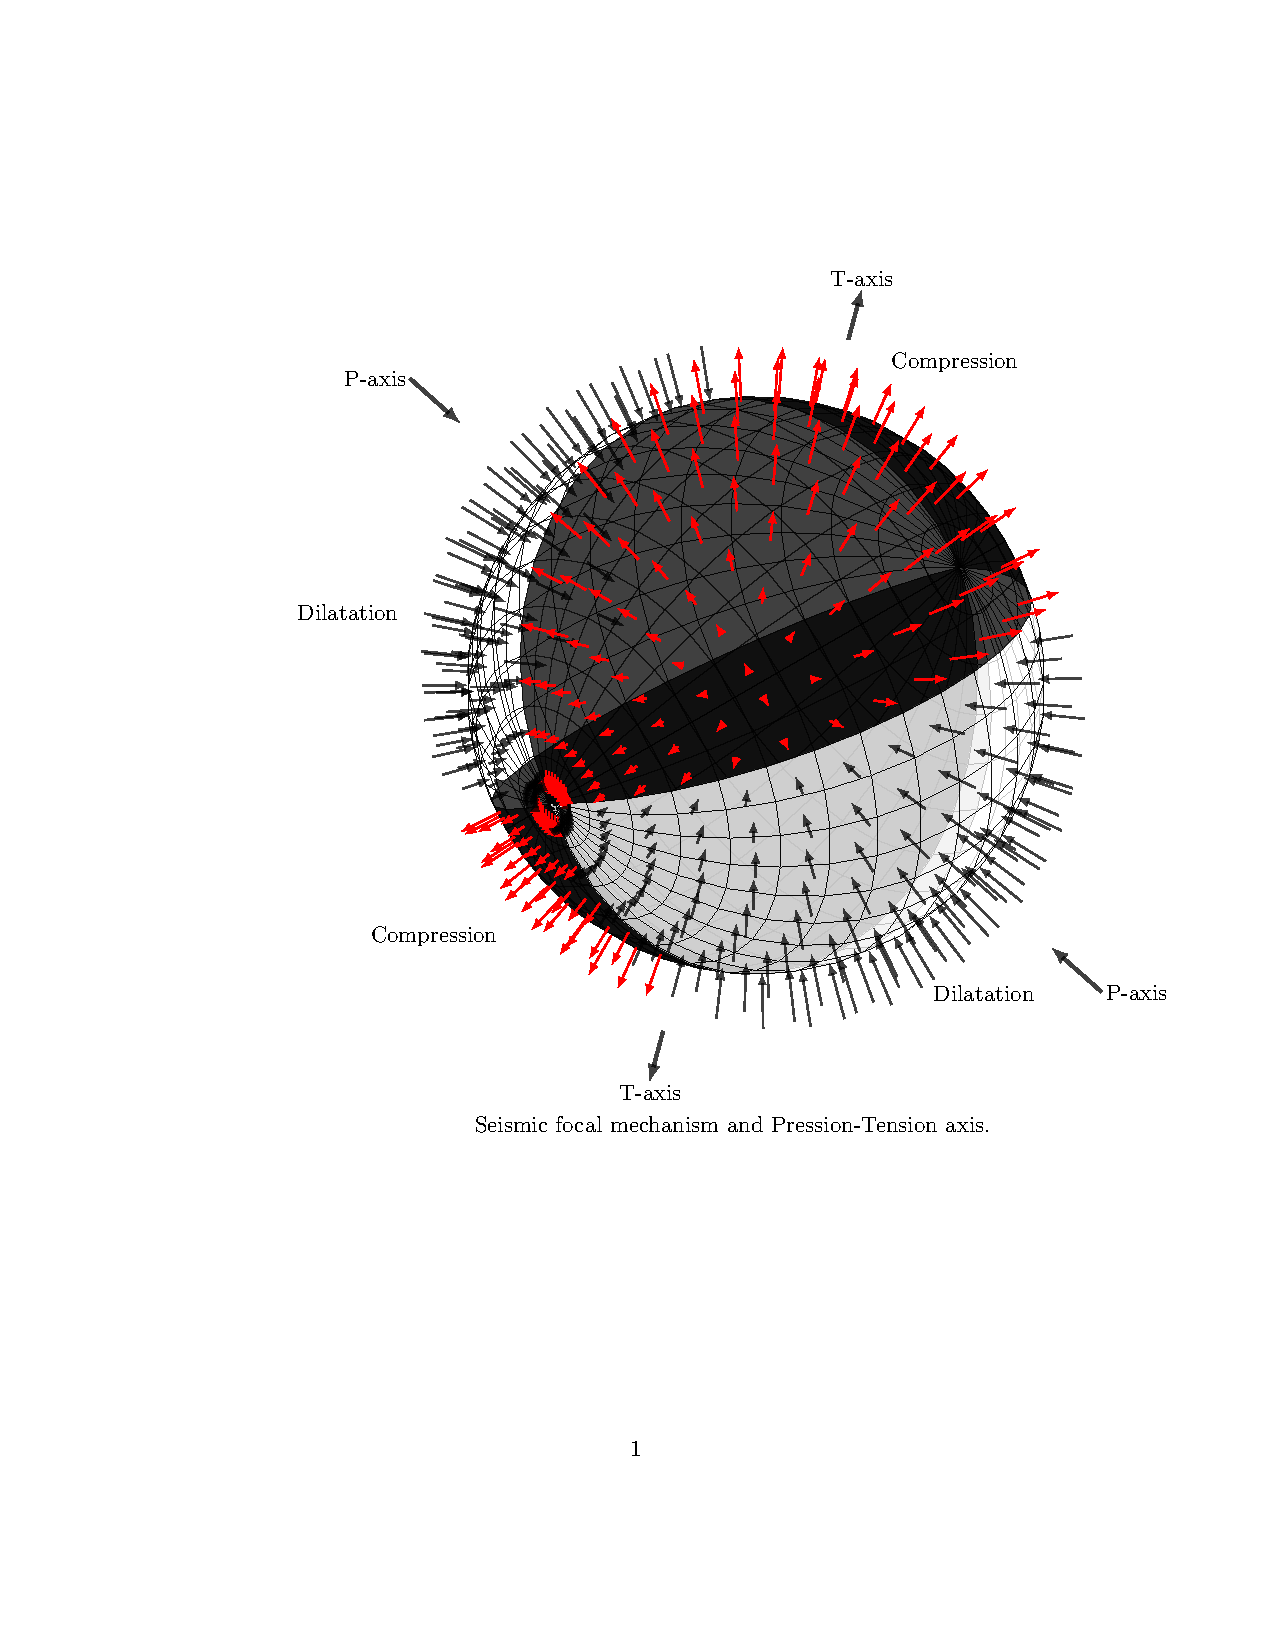
\includegraphics[width=120mm]{SeismicSphere.pdf}
%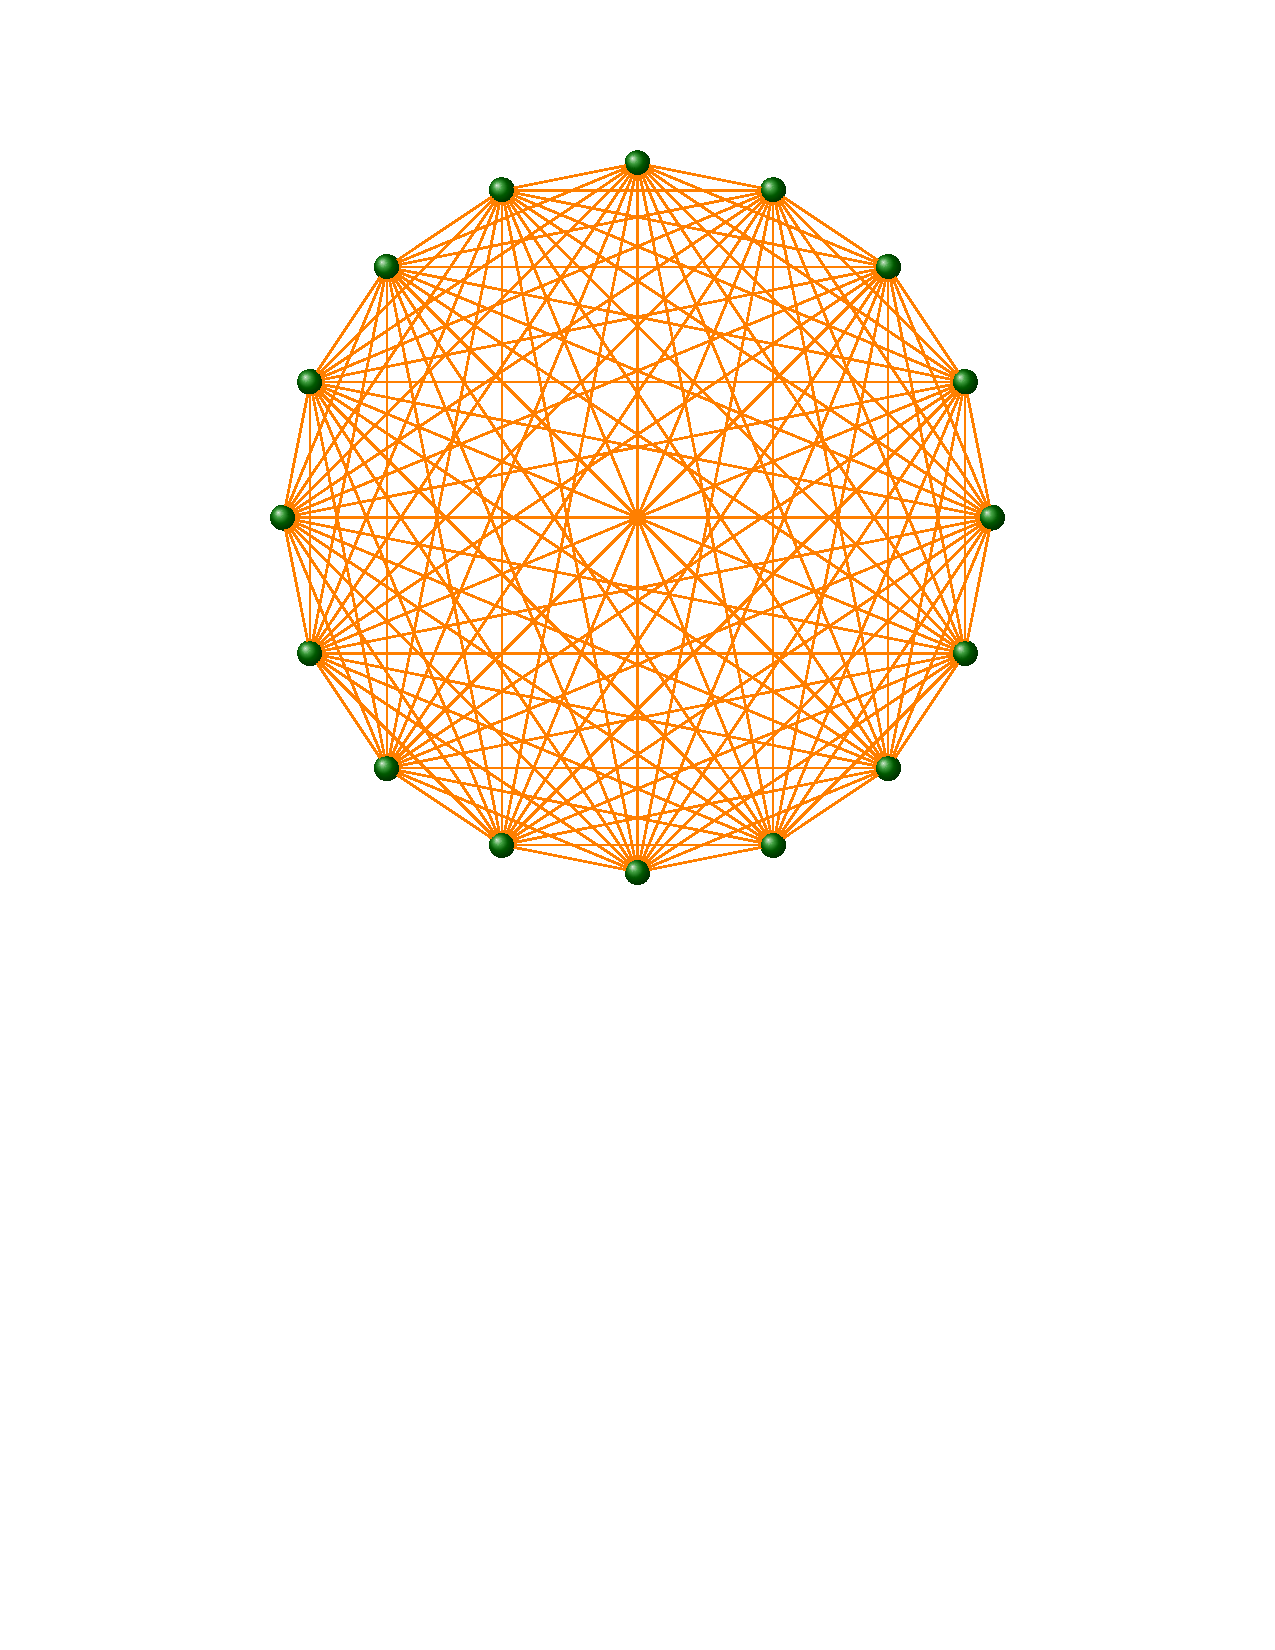
\includepdf[width=50mm]{Circulating-Graph.pdf}

%\subsubsection{Magnetic fields}
%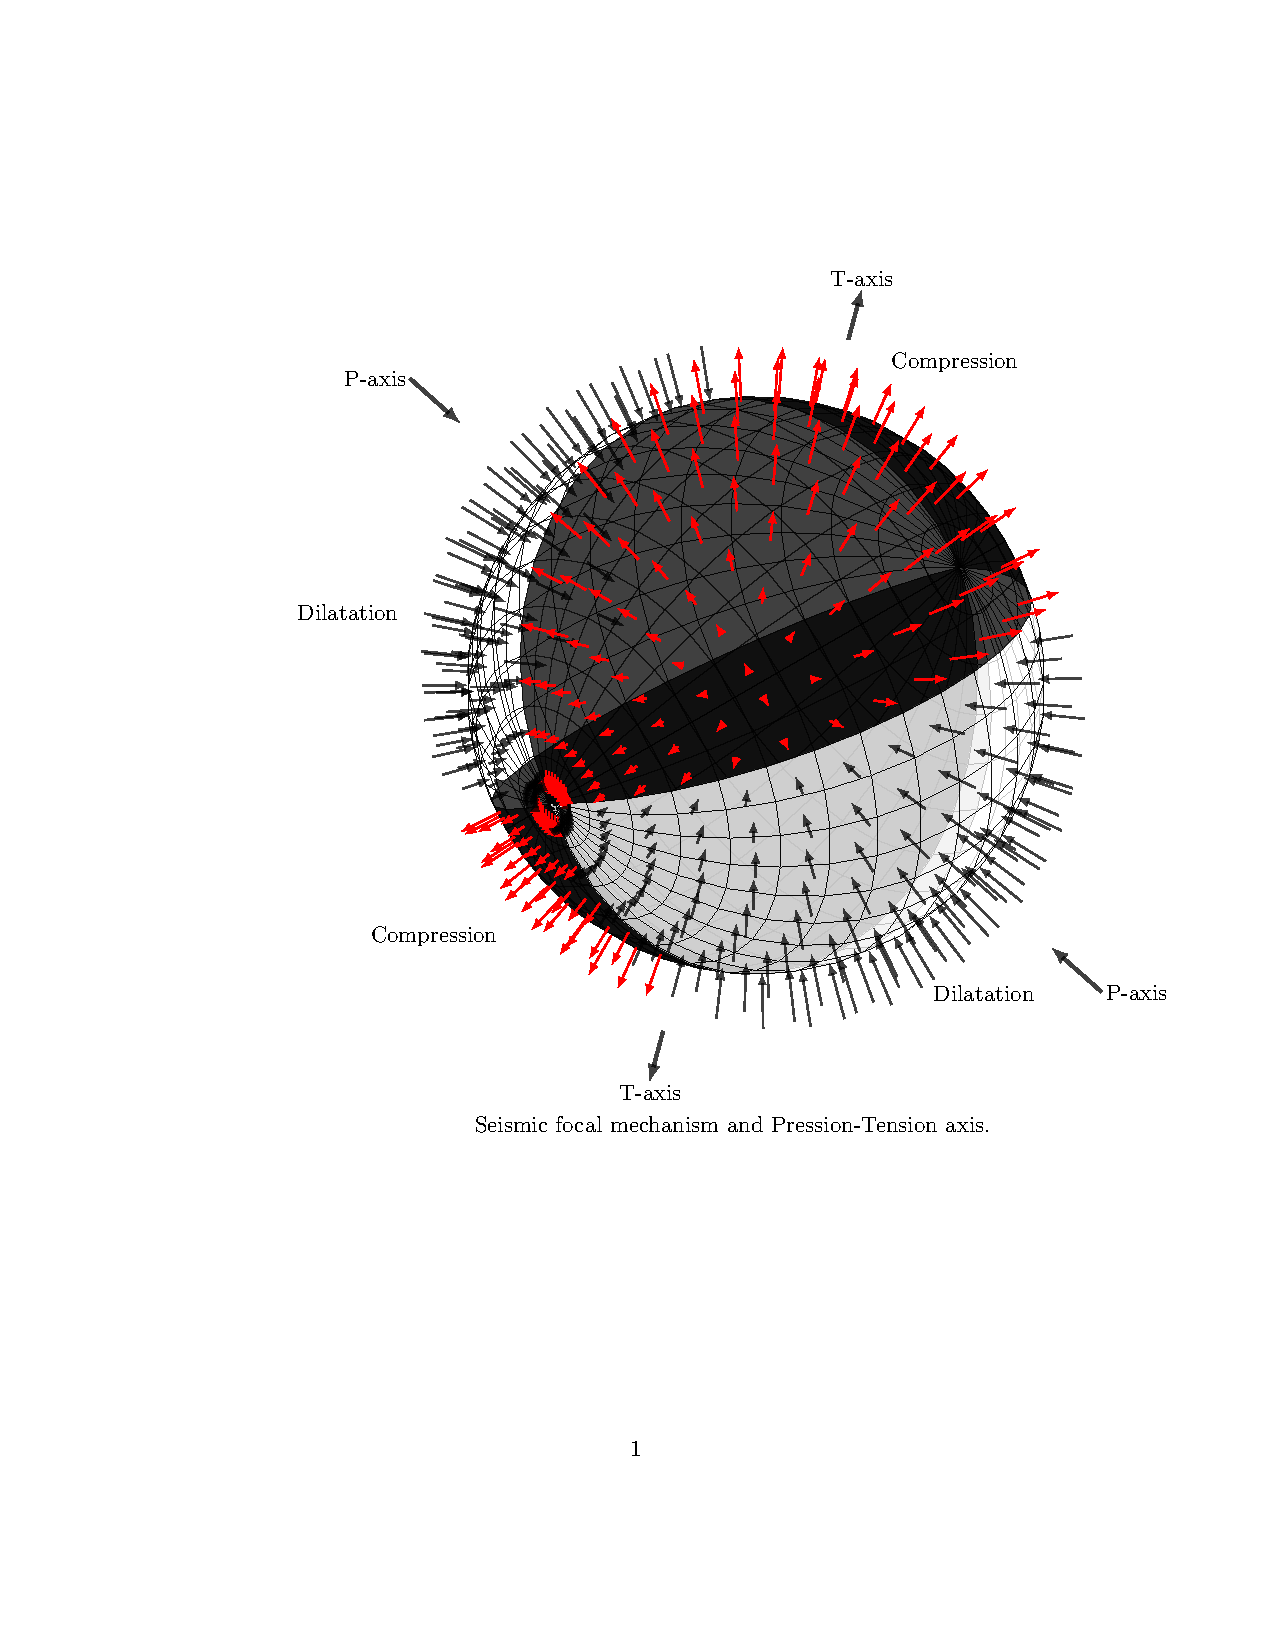
\includegraphics[width=120mm]{SeismicSphere.pdf}
%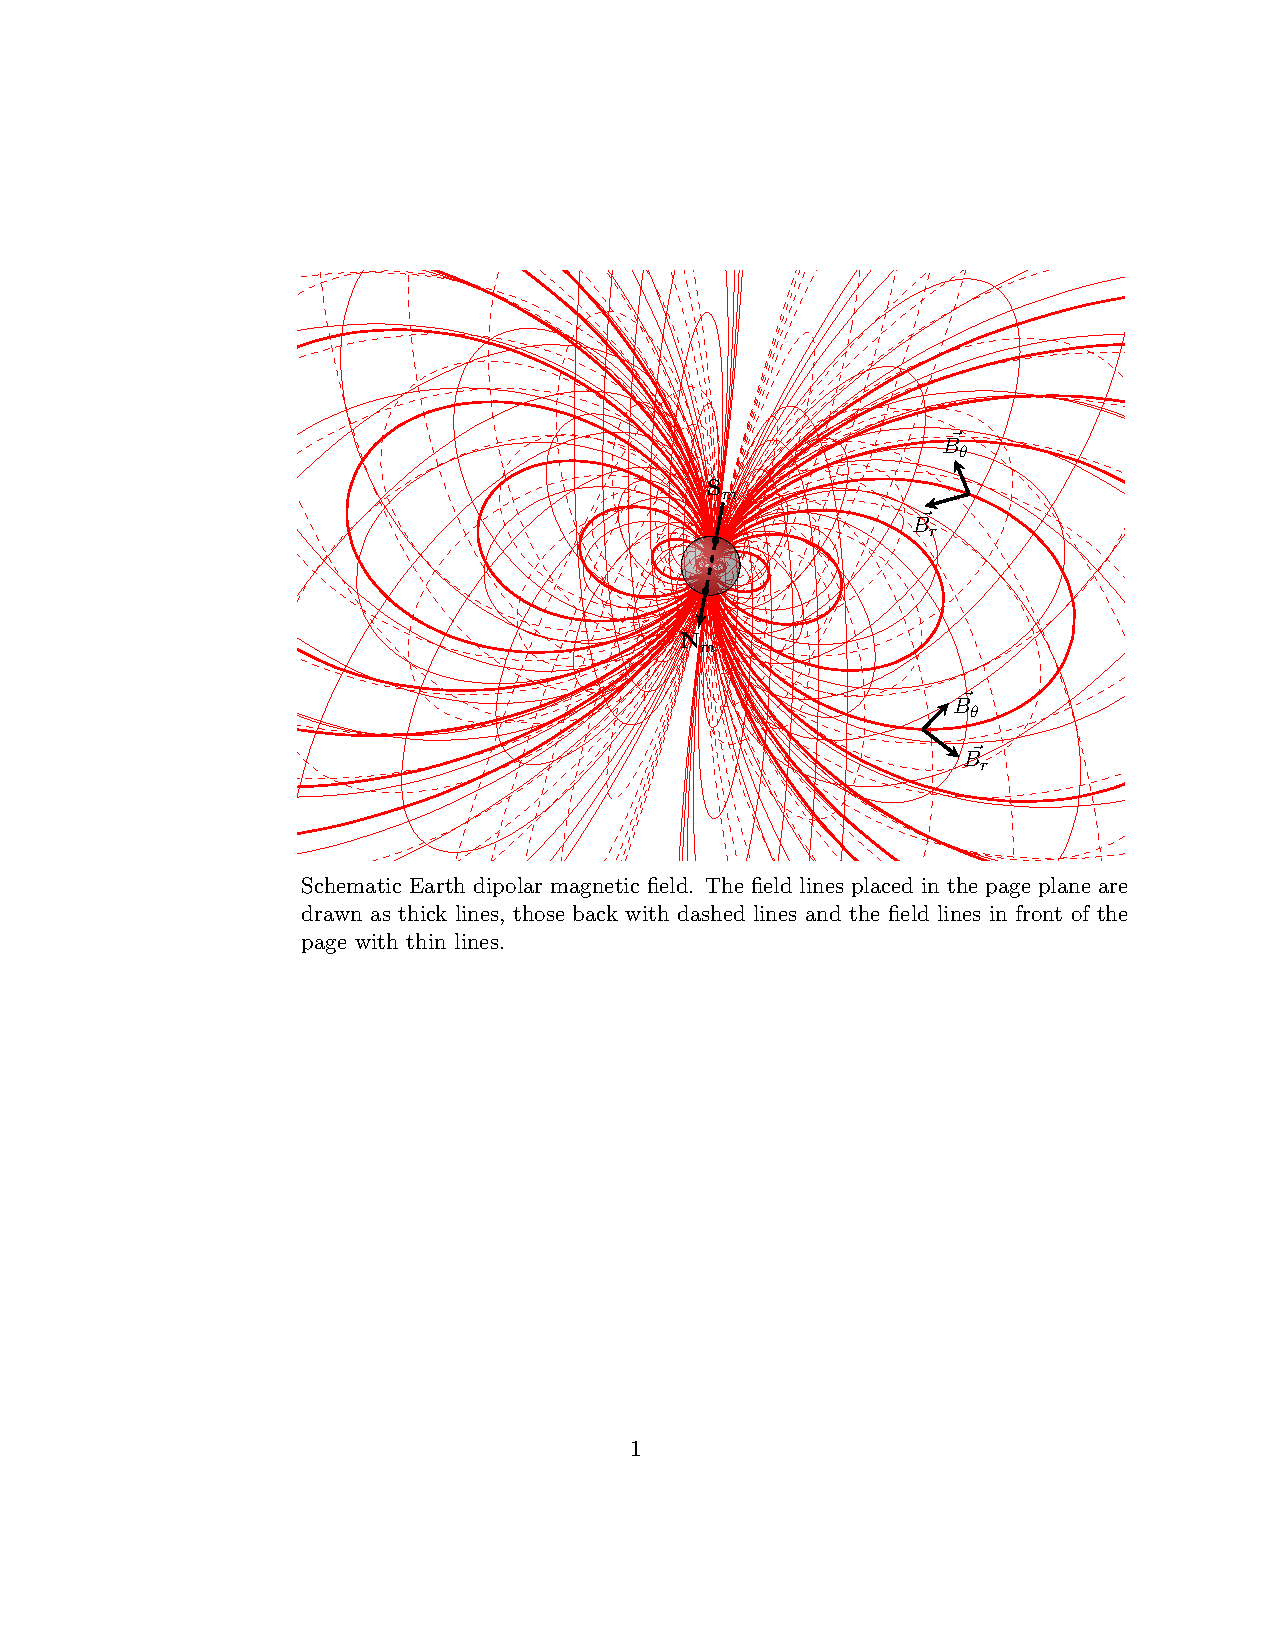
\includepdf[width=50mm]{Magneticfield.pdf}

%\subsubsection{TimeTable}
%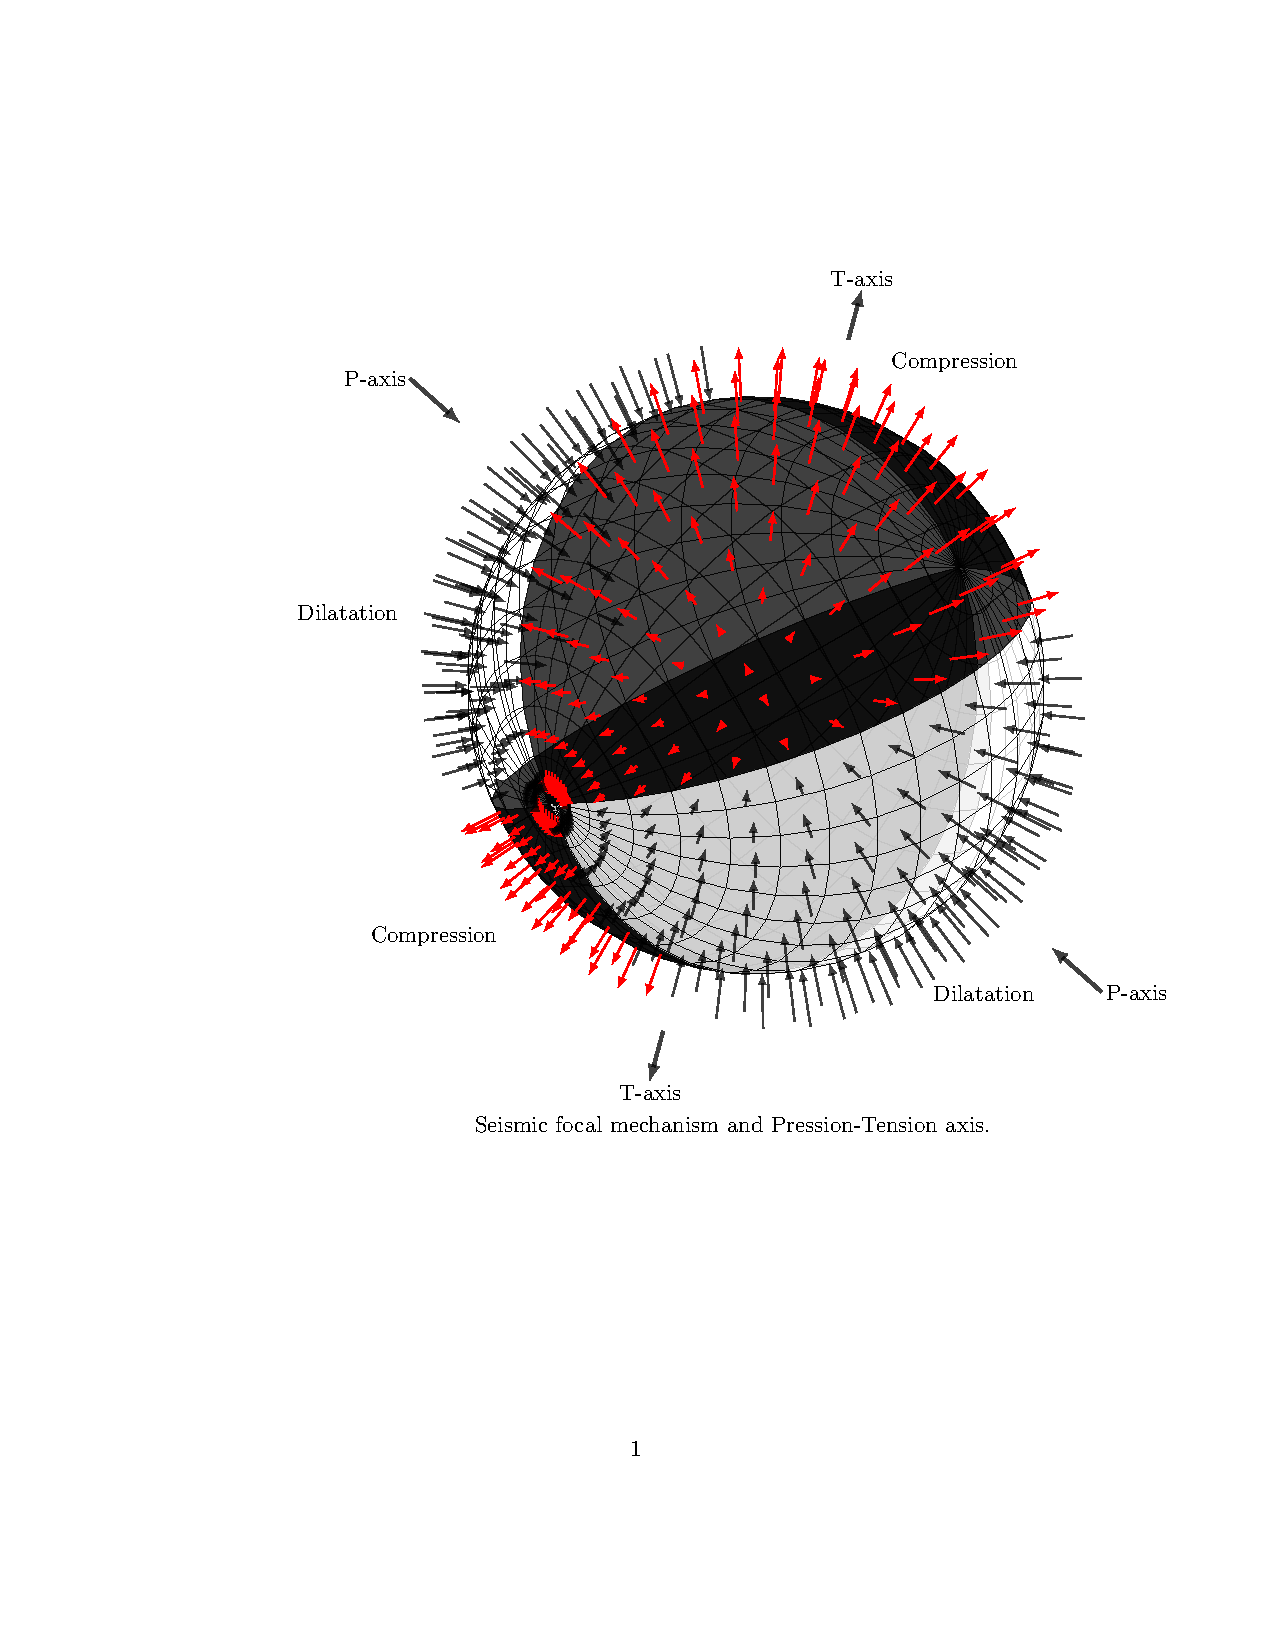
\includegraphics[width=120mm]{SeismicSphere.pdf}
%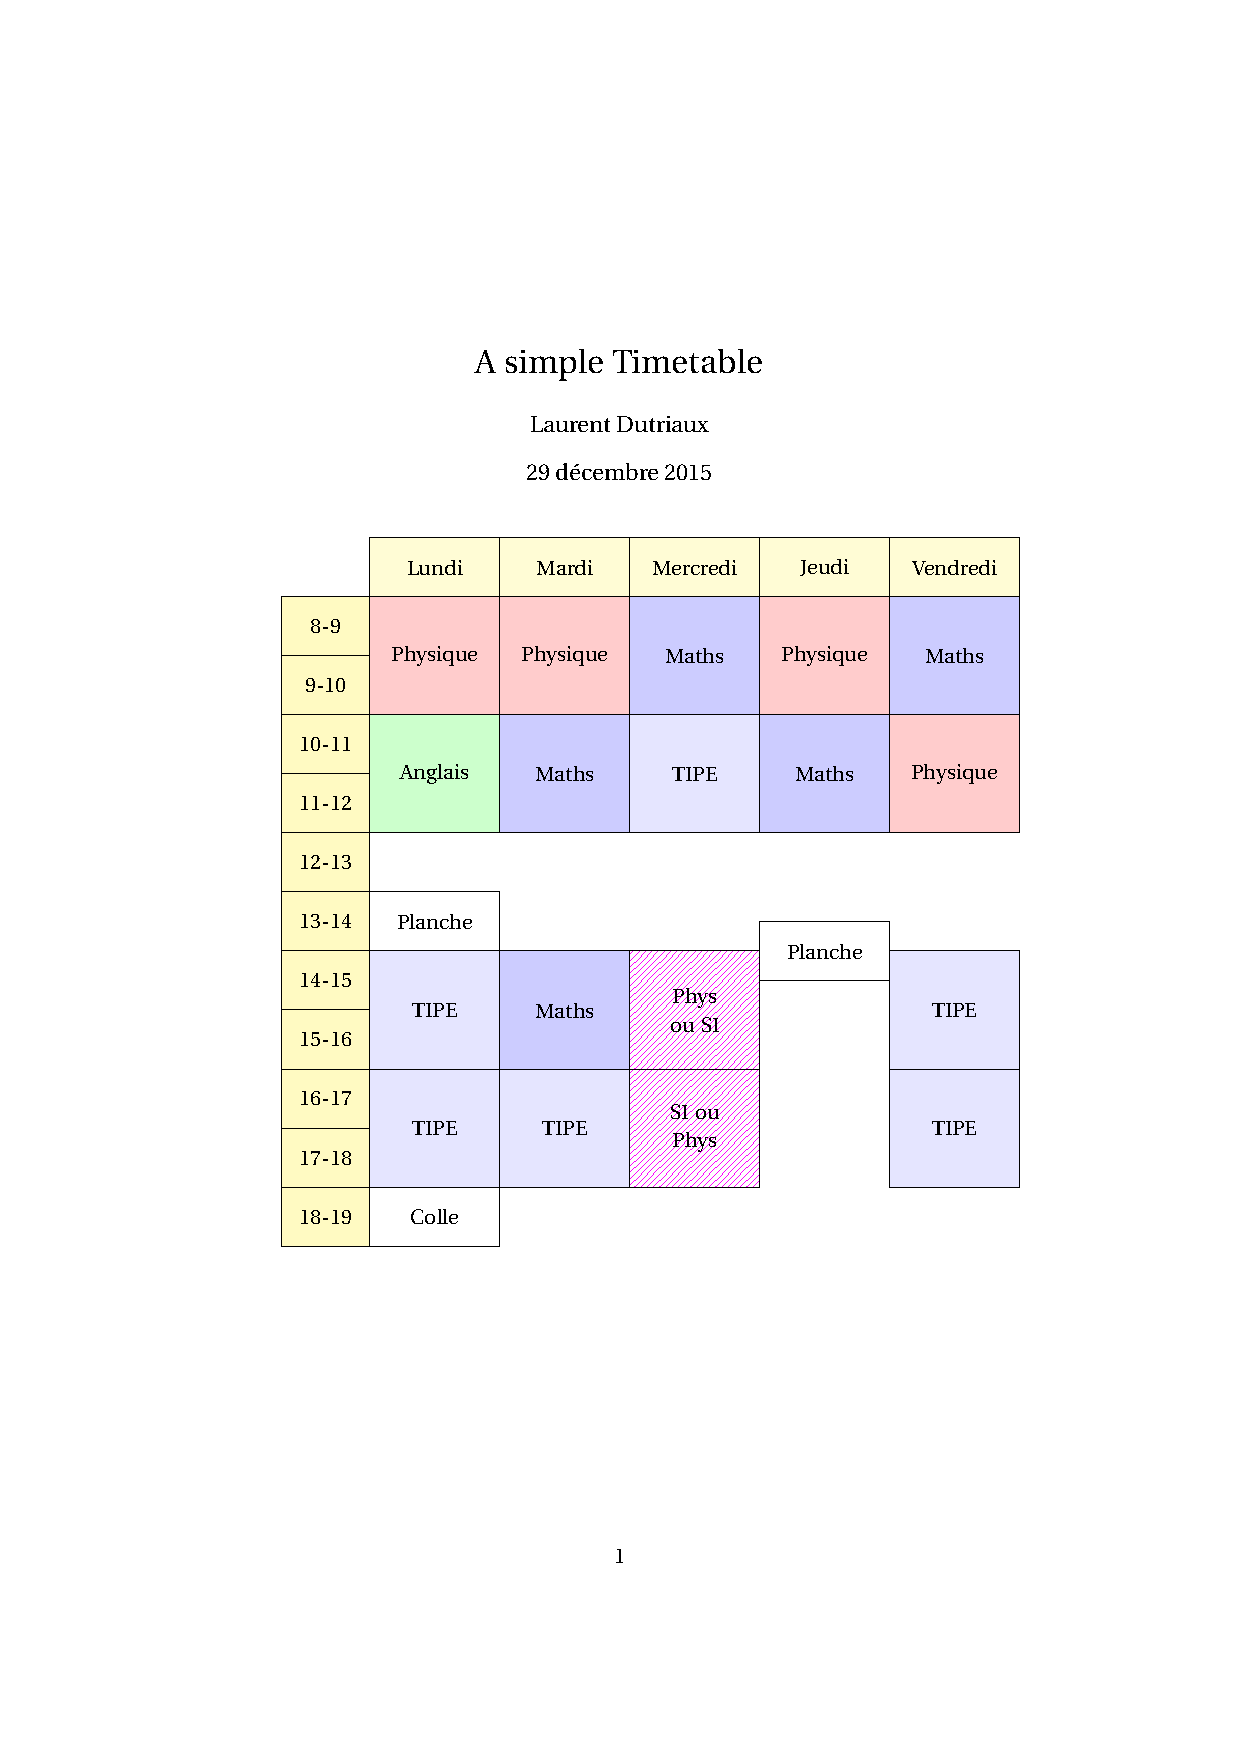
\includepdf[width=50mm]{TimeTable.pdf}

%\subsubsection{Journal de Bord}
%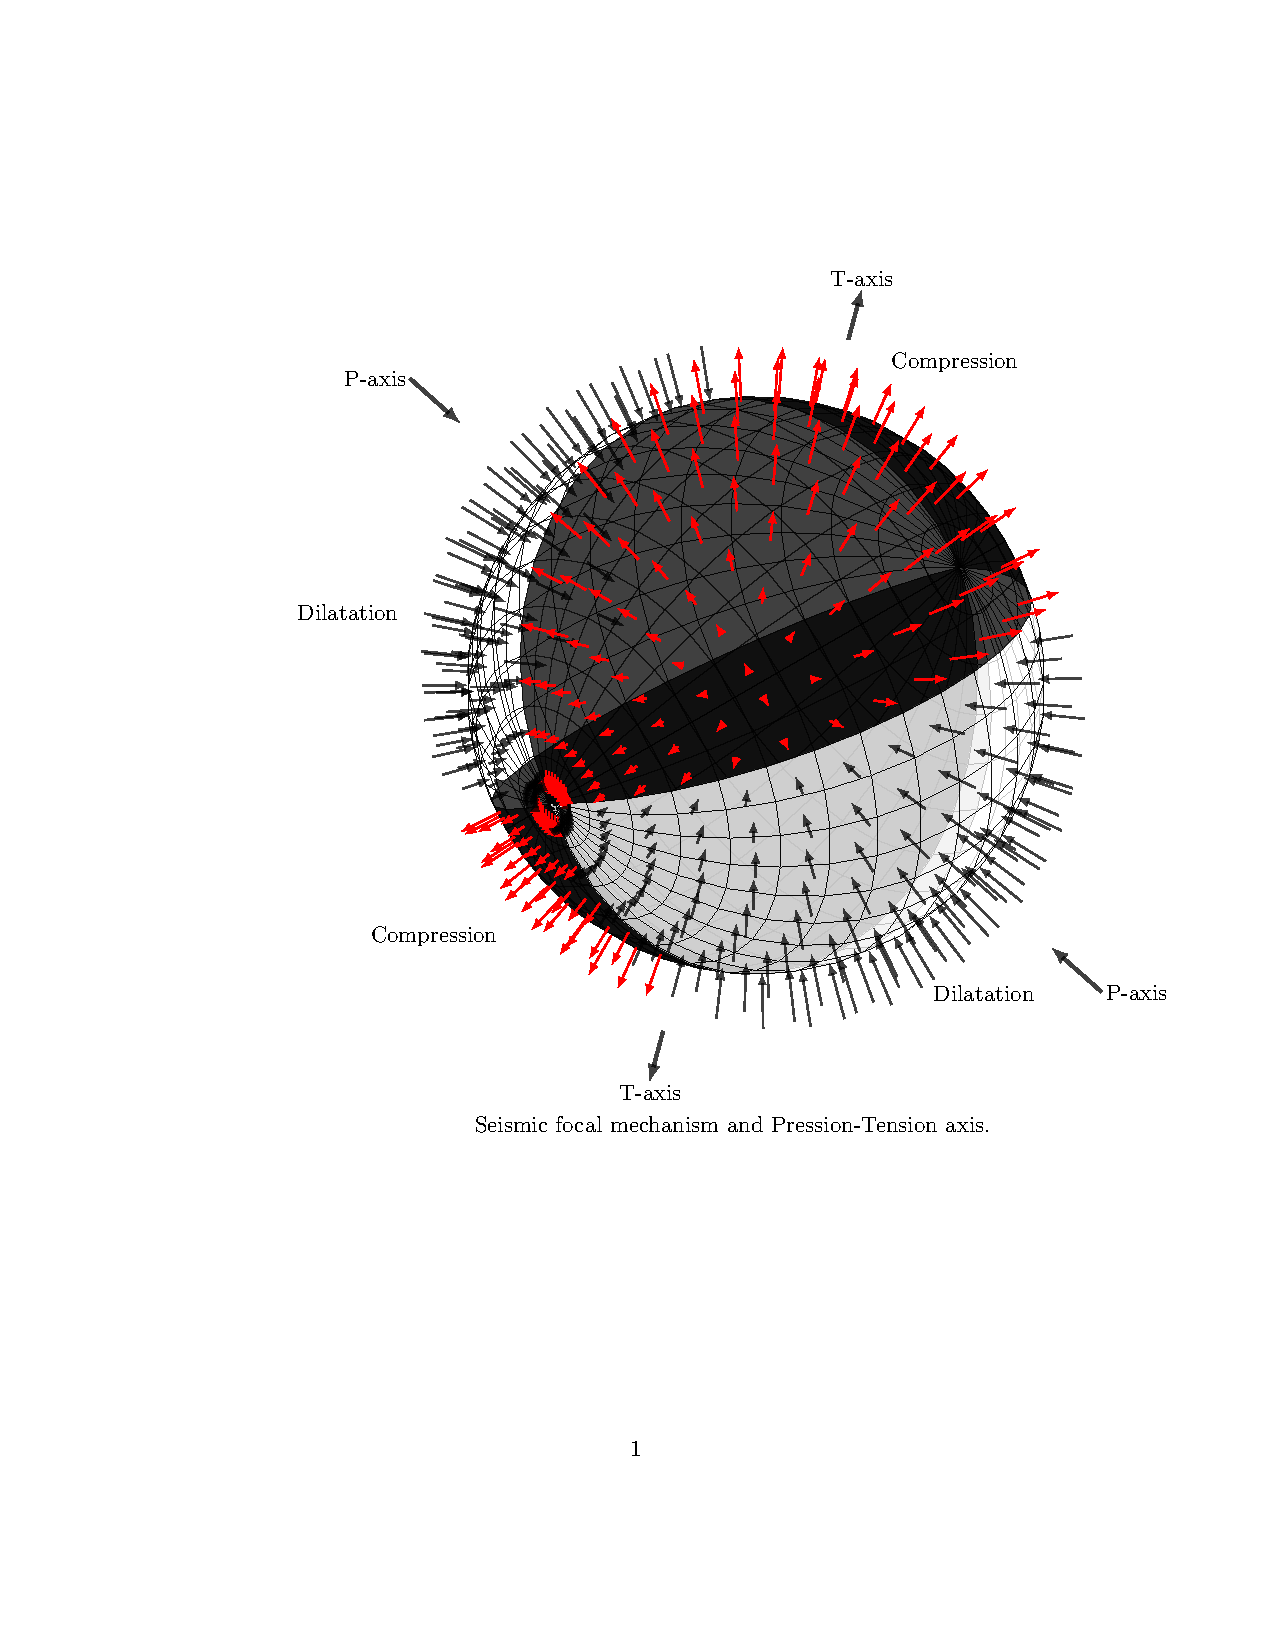
\includegraphics[width=120mm]{SeismicSphere.pdf}
%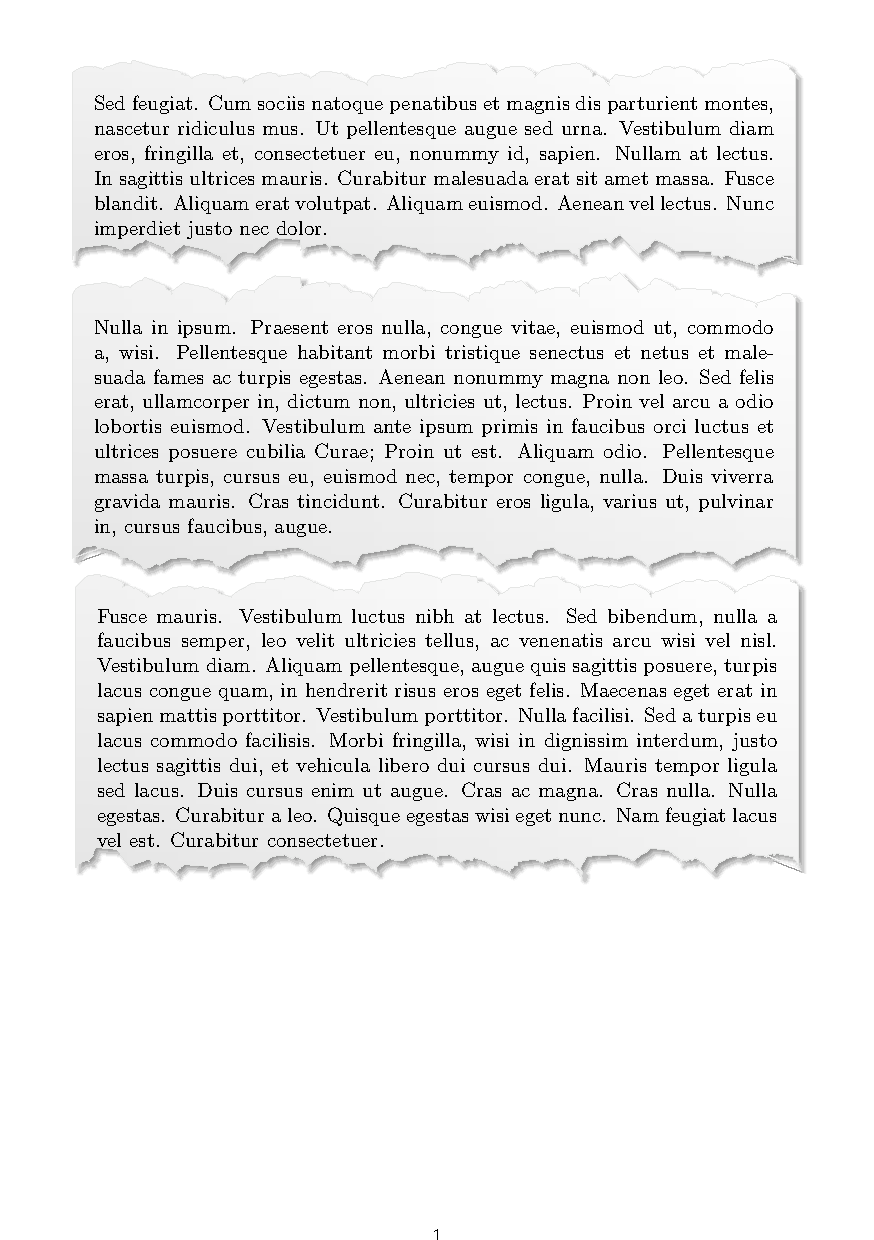
\includepdf[width=50mm]{TornPaper.pdf}

%\subsubsection{Journal de Bord}
%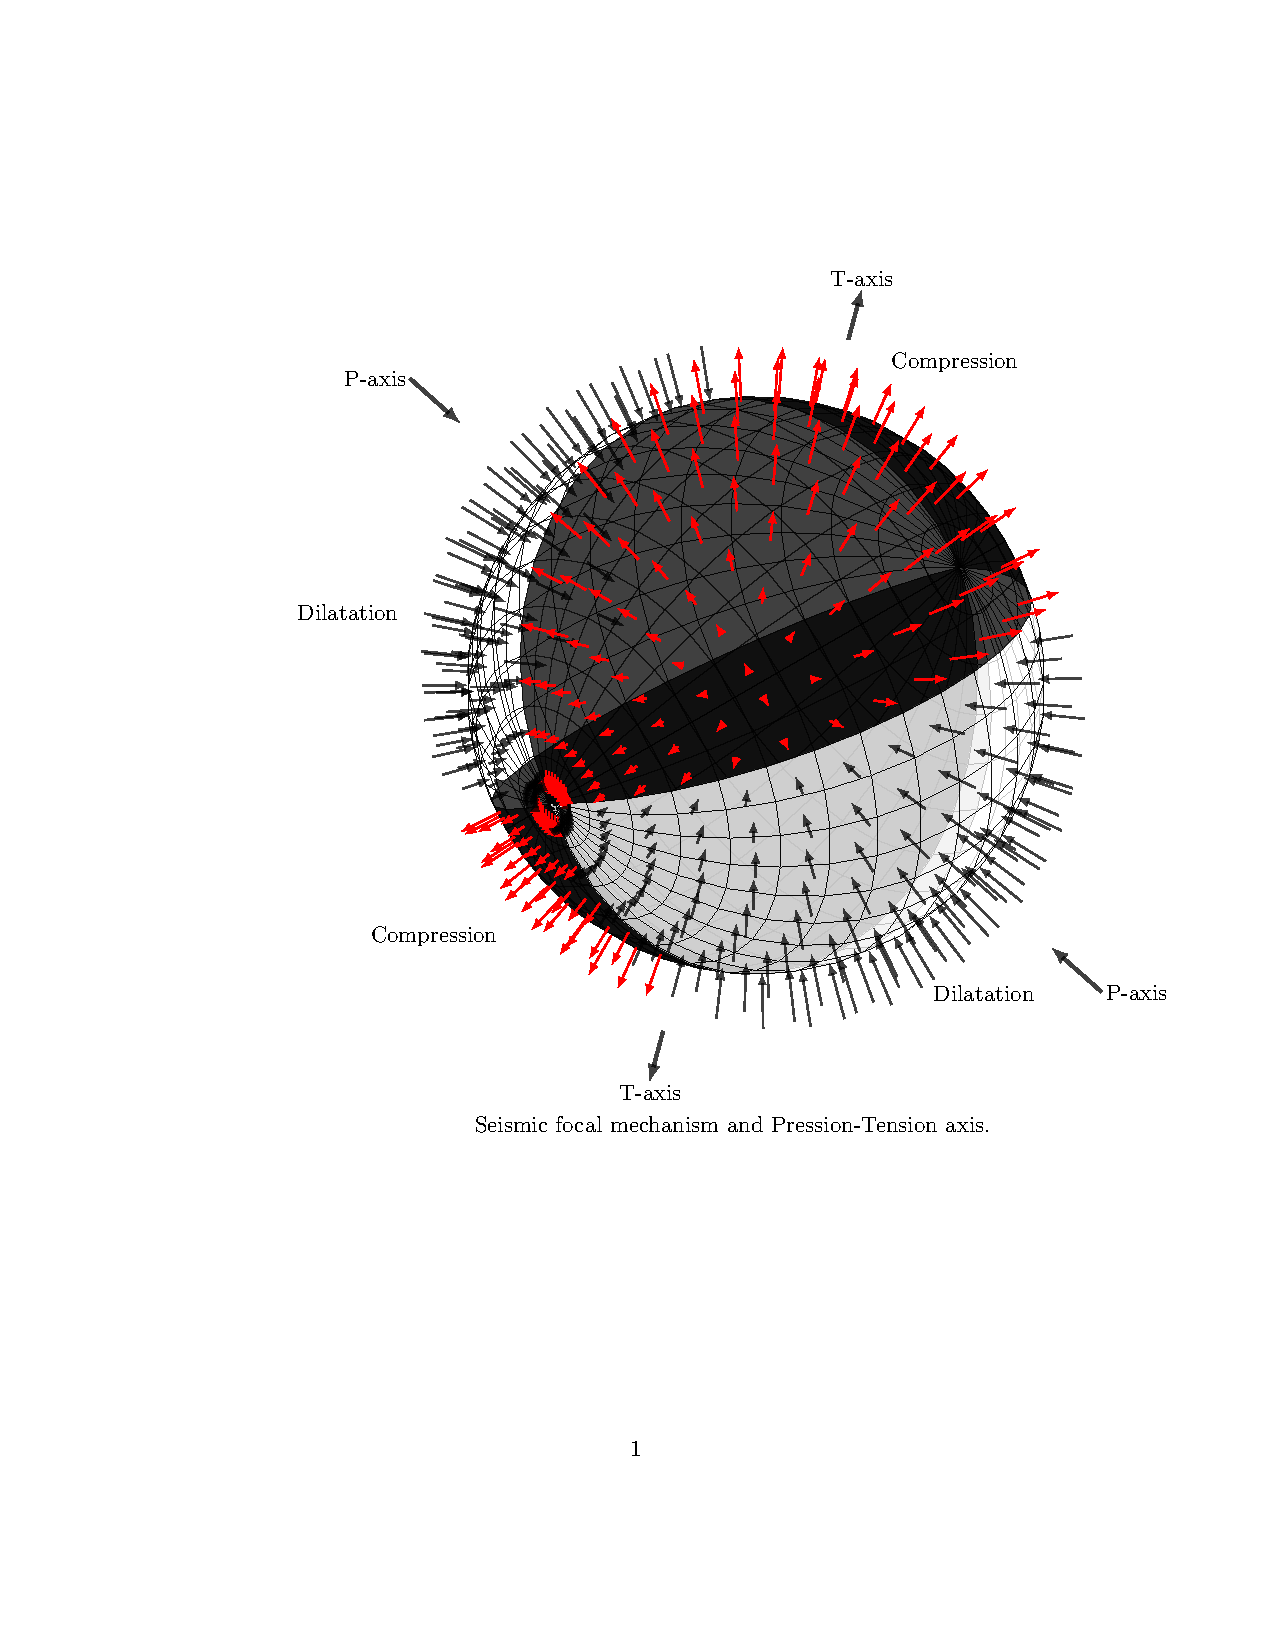
\includegraphics[width=120mm]{SeismicSphere.pdf}
%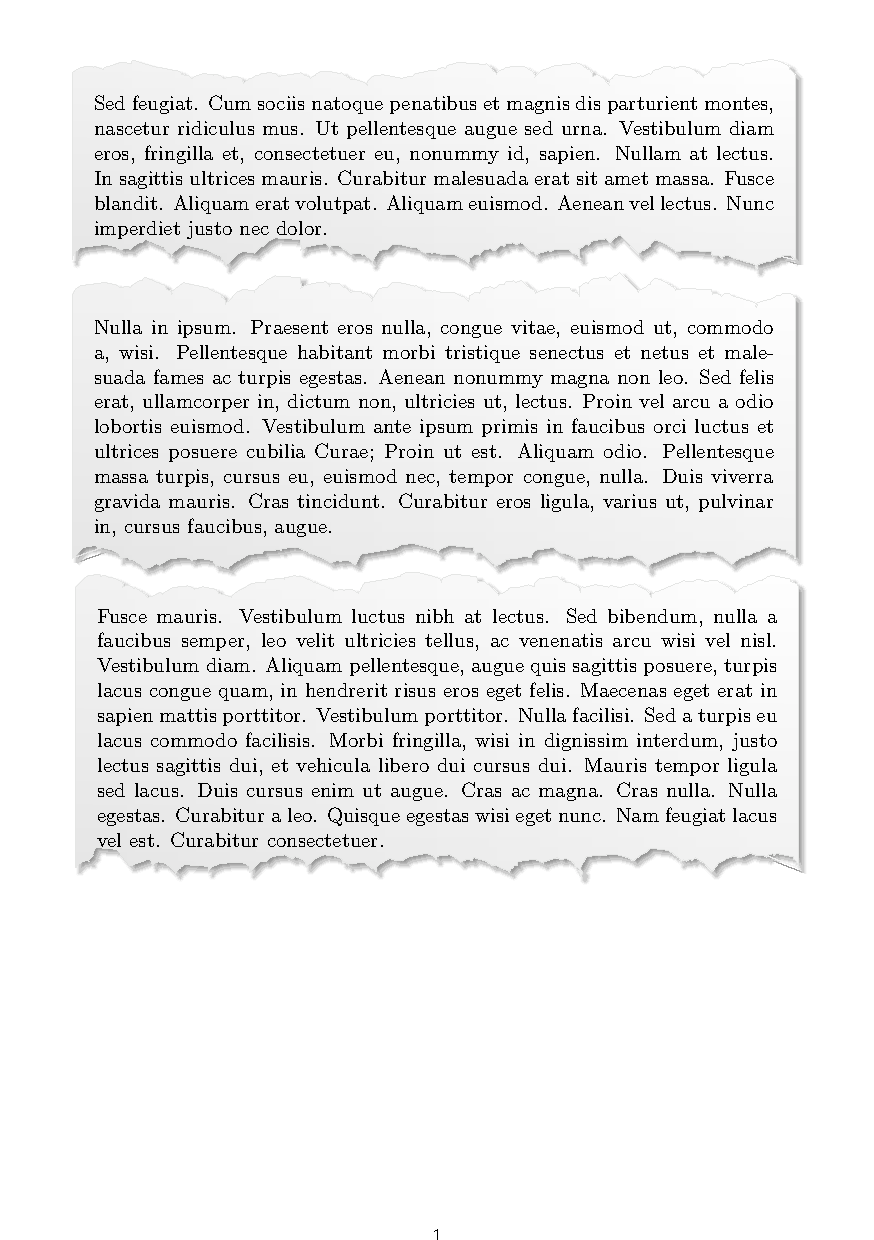
\includepdf{TornPaper.pdf}

\subsection{Weekly calendar}

%{\footnote
%Pour tous les items il faudrait un mail de rappel comme pour les livrables, meetings et vacances
%}

\begin{calendar}{\hsize}

%----------------------------------------------------------------------------------------
%	FIRST DAY
%----------------------------------------------------------------------------------------

\day{}{
09:15-10:15 \daysep \textbf{Messe}\\[3pt]
\textbf{10am-12am} \daysep Marche\\[3pt]
\textbf{12am-2pm} \daysep Dejeuner maison\\[3pt]
\textbf{7pm-9pm} \daysep Canal football club\\[3pt]
\textbf{9pm-11pm} \daysep Guitar\\[3pt]
\textbf{12am-2pm} \daysep Muscu\\[3pt]
}
% By default all daily events are centered in the box, in order to bring them up use \vspace{2cm} after the event text; you may need to change the 2cm

%----------------------------------------------------------------------------------------
%	SECOND DAY
%----------------------------------------------------------------------------------------

\day{}{
\textbf{9am-10am} \daysep Preparation cours de math \\[3pt]
\textbf{10am-12am} \daysep Preparation presentation finance \\[3pt]
\textbf{1pm-2pm} \daysep Manage my weekly \\[3pt]
\textbf{2pm-4pm} \daysep Administration \\[3pt]
\textbf{4pm-5pm} \daysep Lessive \\[3pt]
\textbf{7pm-10pm} \daysep Cinema \\[3pt]
%\textbf{9am-10am} \daysep BIOSCI101 - BLT100 \\[3pt]
%\textbf{10am-11am} \daysep BIOSCI 104 - LLT \\[3pt]
%\textbf{11am-12pm} \daysep No Lecture \\[3pt]
%\textbf{12pm-1pm} \daysep No Lecture \\[3pt]
%\textbf{12pm-1pm} \daysep BIOSCI105 - BLT204 \\[3pt]
%\textbf{1pm-2pm} \daysep No Lecture \\[3pt]
%\textbf{3pm-4pm} \daysep BIOSCI101 Laboratory \\[3pt]
%\textbf{4pm-5pm} \daysep BIOSCI101 Laboratory
} 

%----------------------------------------------------------------------------------------
%	THIRD DAY
%----------------------------------------------------------------------------------------

\day{}{ % Tuesday
\textbf{9am-10am} \daysep Preparation cours de math \\[3pt]
\textbf{10am-12am} \daysep Preparation presentation finance \\[3pt]
\textbf{10am-12am} \daysep Bibliotheque \\[3pt]
\textbf{10am-12am} \daysep Validation of finances\\[3pt]
\textbf{7pm-9pm} \daysep Krav maga \\[3pt]
%\textbf{3pm-4pm} \daysep No Lecture \\[3pt]
%\textbf{4pm-5pm} \daysep No Lecture
} 

%----------------------------------------------------------------------------------------
%	FOURTH DAY
%----------------------------------------------------------------------------------------

\day{}{ % Wednesday
\textbf{9am-10am} \daysep Preparation cours de math \\[3pt]
\textbf{10am-12am} \daysep Preparation presentation finance \\[3pt]
%\textbf{9am-10am} \daysep No Lecture \\[3pt]
%\textbf{10am-11am} \daysep BIOSCI 104 - LLT \\[3pt]
%\textbf{11am-12pm} \daysep No Lecture \\[3pt]
%\textbf{12pm-1pm} \daysep BIOSCI105 - BLT204 \\[3pt]
%\textbf{1pm-2pm} \daysep No Lecture \\[3pt]
%\textbf{2pm-3pm} \daysep GEO101 - HSB1 \\[3pt]
\textbf{7pm-10pm} \daysep Football \\[3pt]
%\textbf{3pm-4pm} \daysep No Lecture \\[3pt]
%\textbf{4pm-5pm} \daysep No Lecture
} 

%----------------------------------------------------------------------------------------
%	FIFTH DAY
%----------------------------------------------------------------------------------------

\day{}{ % Thursday
\textbf{9am-10am} \daysep Preparation cours de math \\[3pt]
\textbf{10am-12am} \daysep Preparation presentation finance \\[3pt]
\textbf{7pm-9pm} \daysep Krav maga \\[3pt]
%\textbf{9am-10am} \daysep No Lecture \\[3pt]
%\textbf{10am-11am} \daysep BIOSCI 104 - LLT \\[3pt]
%\textbf{11am-12pm} \daysep No Lecture \\[3pt]
%\textbf{12pm-1pm} \daysep No Lecture \\[3pt]
%\textbf{1pm-2pm} \daysep No Lecture \\[3pt]
%\textbf{2pm-3pm} \daysep GEO101 - HSB1 \\[3pt]
%\textbf{3pm-4pm} \daysep No Lecture \\[3pt]
%\textbf{4pm-5pm} \daysep No Lecture
} 

%----------------------------------------------------------------------------------------
%	SIXTH DAY
%----------------------------------------------------------------------------------------

\day{}{ % Friday
\textbf{9am-10am} \daysep Preparation cours de math \\[3pt]
\textbf{10am-12am} \daysep Preparation presentation finance \\[3pt]
\textbf{12am-2pm} \daysep Badminton \\[3pt]
\textbf{9pm-11pm} \daysep Drinks \\[3pt]
%\textbf{10am-11am} \daysep BIOSCI 104 - LLT \\[3pt]
%\textbf{11am-12pm} \daysep No Lecture \\[3pt]
%\textbf{12pm-1pm} \daysep BIOSCI105 - BLT204 \\[3pt]
%\textbf{1pm-2pm} \daysep No Lecture \\[3pt]
%\textbf{2pm-3pm} \daysep No Lecture \\[3pt]
%\textbf{3pm-4pm} \daysep GEO101 Tutorial \\ Room A \\[3pt]
%\textbf{4pm-5pm} \daysep No Lecture
} 

%----------------------------------------------------------------------------------------
%	SEVENTH DAY
%----------------------------------------------------------------------------------------

\day{}{ % Saturday
\textbf{9am-10am} \daysep Preparation cours de math \\[3pt]
\textbf{10am-12am} \daysep Courses \\[3pt]
\textbf{2pm-4pm} \daysep Menage \\[3pt]
\textbf{4pm-9pm} \daysep Get back energy \\[3pt]
\textbf{9pm-11pm} \daysep Go dancing \\[3pt]
\textbf{9pm-11pm} \daysep Go sailing \\[3pt]
}
%----------------------------------------------------------------------------------------
 
\finishCalendar
\end{calendar}

\subsection{Communication}
\begin{itemize}
  \item Il faut que je surveille mon petit canard, pour savoir s'il part pour les migrations ou bien s'il reste à Dinan pour grandir encore un peu.
  \item Nettoyer le lave-vaisselle
  \item Nettoyer le fond du bateau, et les toilettes \ldots
\end{itemize}

\section{Calendar}

\subsection{Events}
{\footnotesize
Only the Birthdays, Deliverables and Meetings for the next 3 days will appear in this list\\
}
{\footnotesize
\begin{longtable}{|c|c|c|c|}
\hline
\multicolumn{4}{|c|}{Events} \\
\hline
Date & Type & Name & Template\\
\hline
Monday January 2013 & Deliverable & Inception & \\
\hline
Monday January 2013 & Deliverable & Specification & \\
\hline
Monday January 2013 & Deliverable & Clearchoice & \\
\hline
Monday January 2013 & Deliverable & External design & \\
\hline
Monday January 2013 & Deliverable & Internal design & \\
\hline
Monday January 2013 & Deliverable & Test documentation & \\
\hline
Monday January 2013 & Deliverable & Release notes & \\
\hline
Monday January 2013 & Deliverable & Post implementation review & \\
\hline
Monday January 2013 & Deliverable & Support documentation & \\
\hline
Monday January 2013 & Deliverable & Inception & \\
\hline
Monday January 2013 & Deliverable & Specification & \\
\hline
Monday January 2013 & Deliverable & Clearchoice & \\
\hline
Monday January 2013 & Deliverable & External design & \\
\hline
Monday January 2013 & Deliverable & Internal design & \\
\hline
Monday January 2013 & Deliverable & Test documentation & \\
\hline
Monday January 2013 & Deliverable & Release notes & \\
\hline
Monday January 2013 & Deliverable & Post implementation review & \\
\hline
Saturday November 2013 & Deliverable & Support documentation & \\
\hline
Friday November 2013 & Birthday & Annif Antoine & \\
\hline
Thursday October 2013 & Meeting & Council & Council.tex\\
\hline
Wednesday June 2014 & Meeting & Council & Council.tex\\
\hline
Monday December 2015 & Daily & Daily setup & ManagementSummary.pdf\\
\hline
Monday December 2015 & Daily & Daily setup & ManagementSummary.pdf\\
\hline
Monday December 2015 & Event & Renouvellement Assu Auto & Letter.pdf\\
\hline
Sunday December 2015 & Event & Renouvellement Assu Bateau & Letter.pdf\\
\hline
Sunday December 2015 & Event & Renouvellement Assu Maison & Letter.pdf\\
\hline
Saturday December 2015 & Event & Revision auto & Letter.pdf\\
\hline
Saturday December 2015 & Event & Renouvellement carte paiement & Letter.pdf\\
\hline
Friday December 2015 & Event & Declaration impots & Letter.pdf\\
\hline
Friday December 2015 & Event & Paiement des impots & Letter.pdf\\
\hline
Thursday December 2015 & Event & Arbre de noel & Letter.pdf\\
\hline
 ... & ... & ... & ... \\
\hline
\hline
\end{longtable}

}

\subsection{Contacts for the events}
{\footnotesize
Only contacts linked to the Birthdays, Deliverables and Meetings for the next 3 days will appear in this list\\
\begin{longtable}{|c|c|c|}
\hline
\multicolumn{3}{|c|}{Contacts} \\
\hline
Name & Email & Telephone\\
\hline
\end{longtable}

%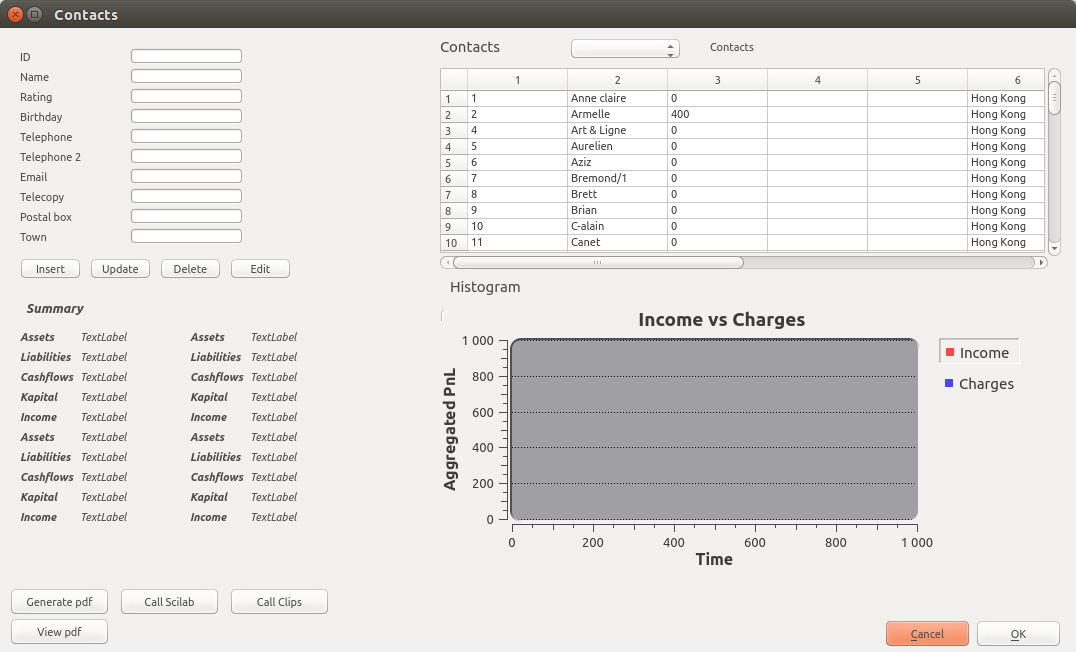
\includegraphics[width=20mm]{Contacts.png}
%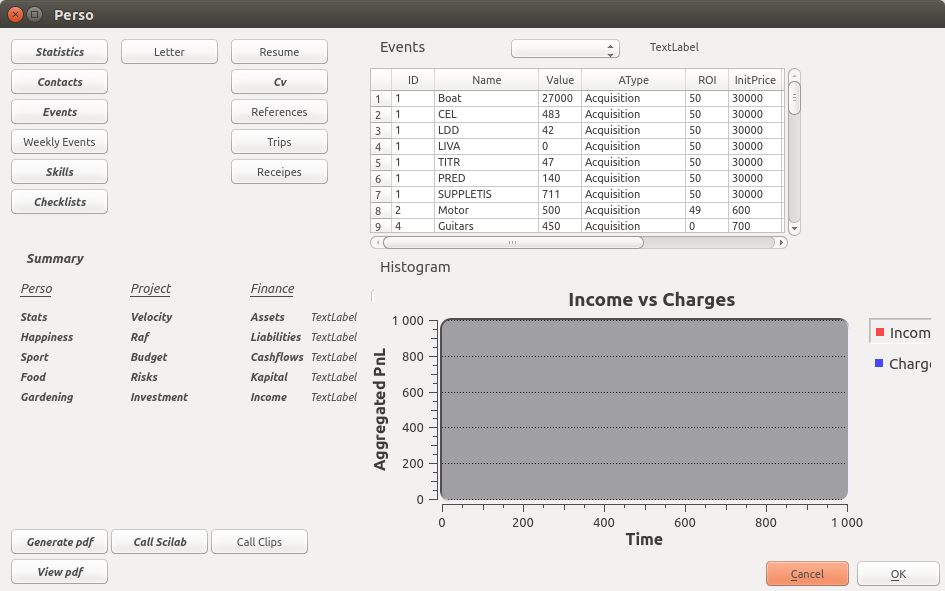
\includegraphics[width=20mm]{Perso.png}
%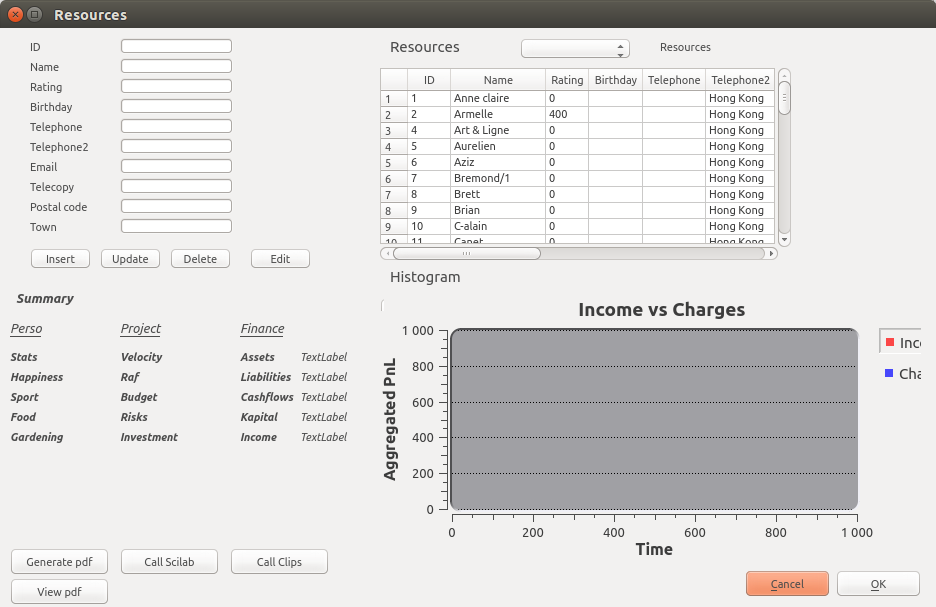
\includegraphics[width=20mm]{Resources.png}
%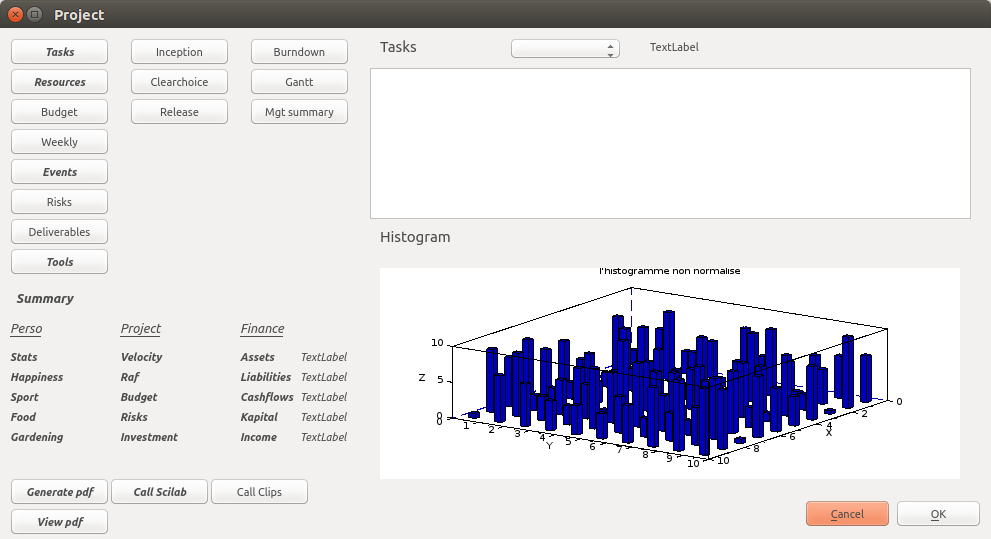
\includegraphics[width=20mm]{Projects.png}
%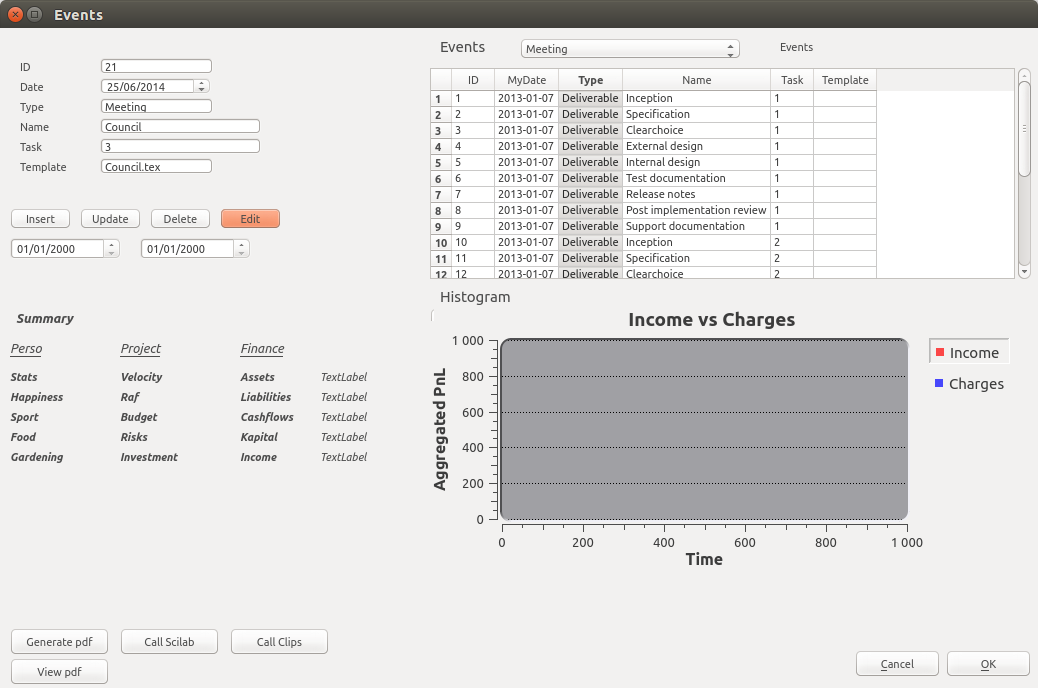
\includegraphics[width=20mm]{Events.png}
%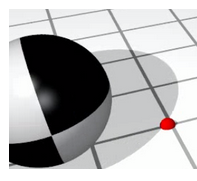
\includegraphics[width=10mm]{Logo.png}
%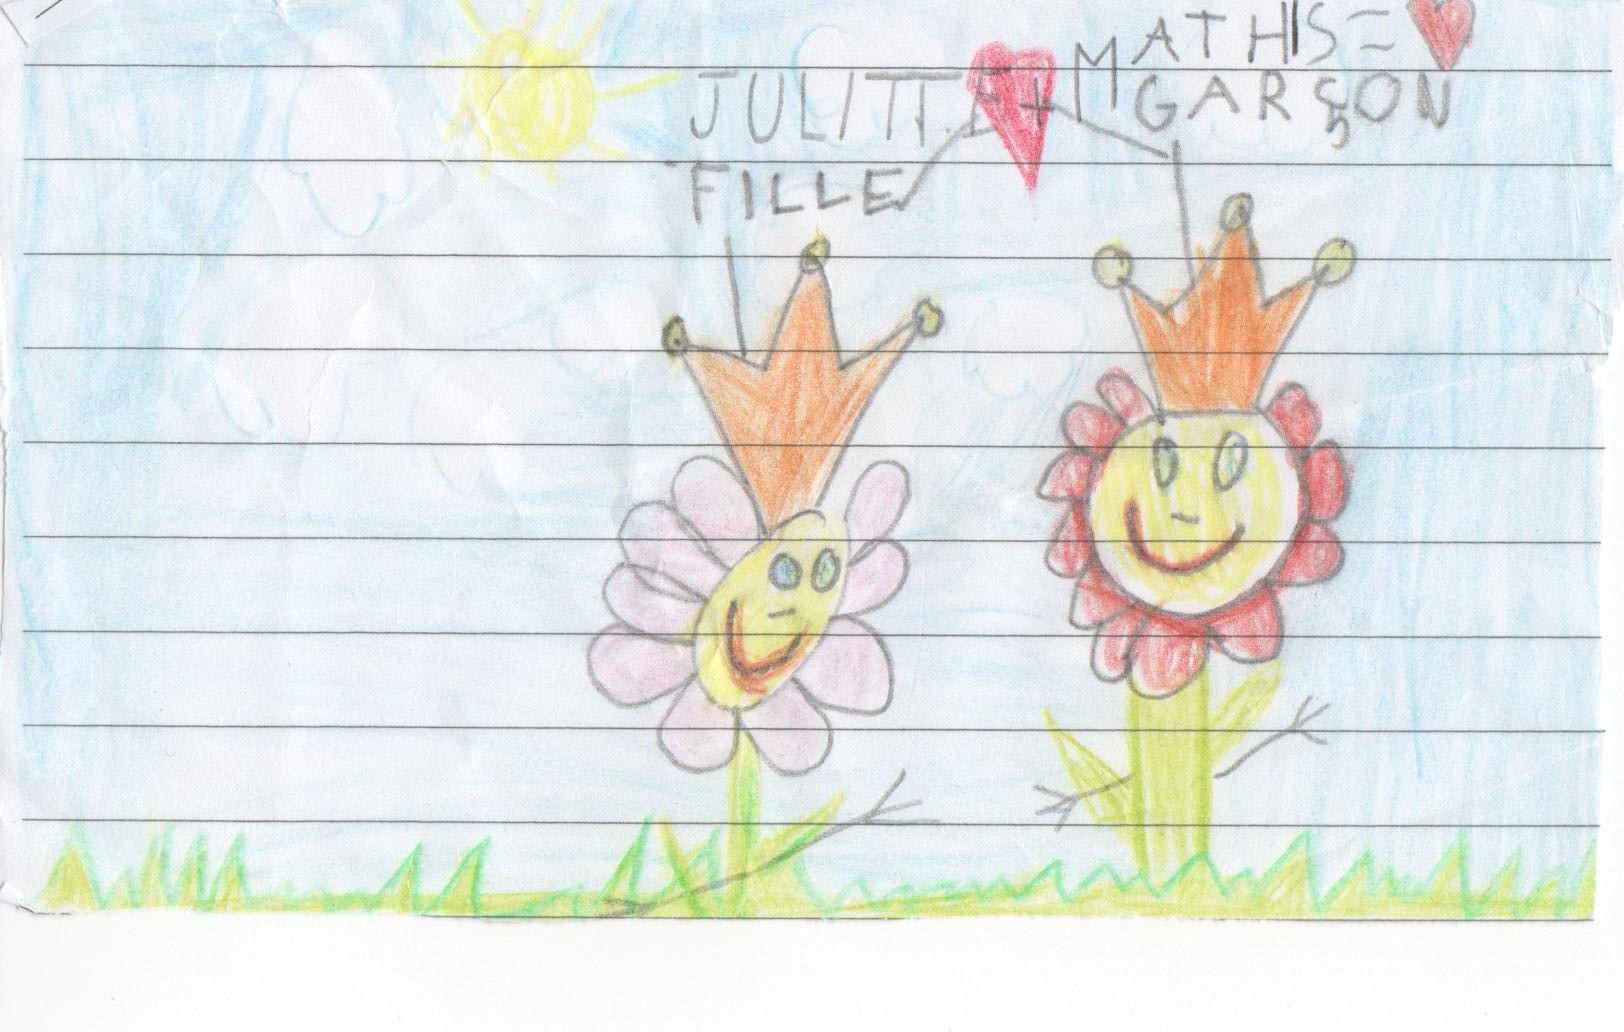
\includegraphics[width=10mm]{011.jpg}
}
\begin{itemize}
  \item Contact1 
  \item Contact2 
  \item Contact3 
\end{itemize}

\section{Resume}
%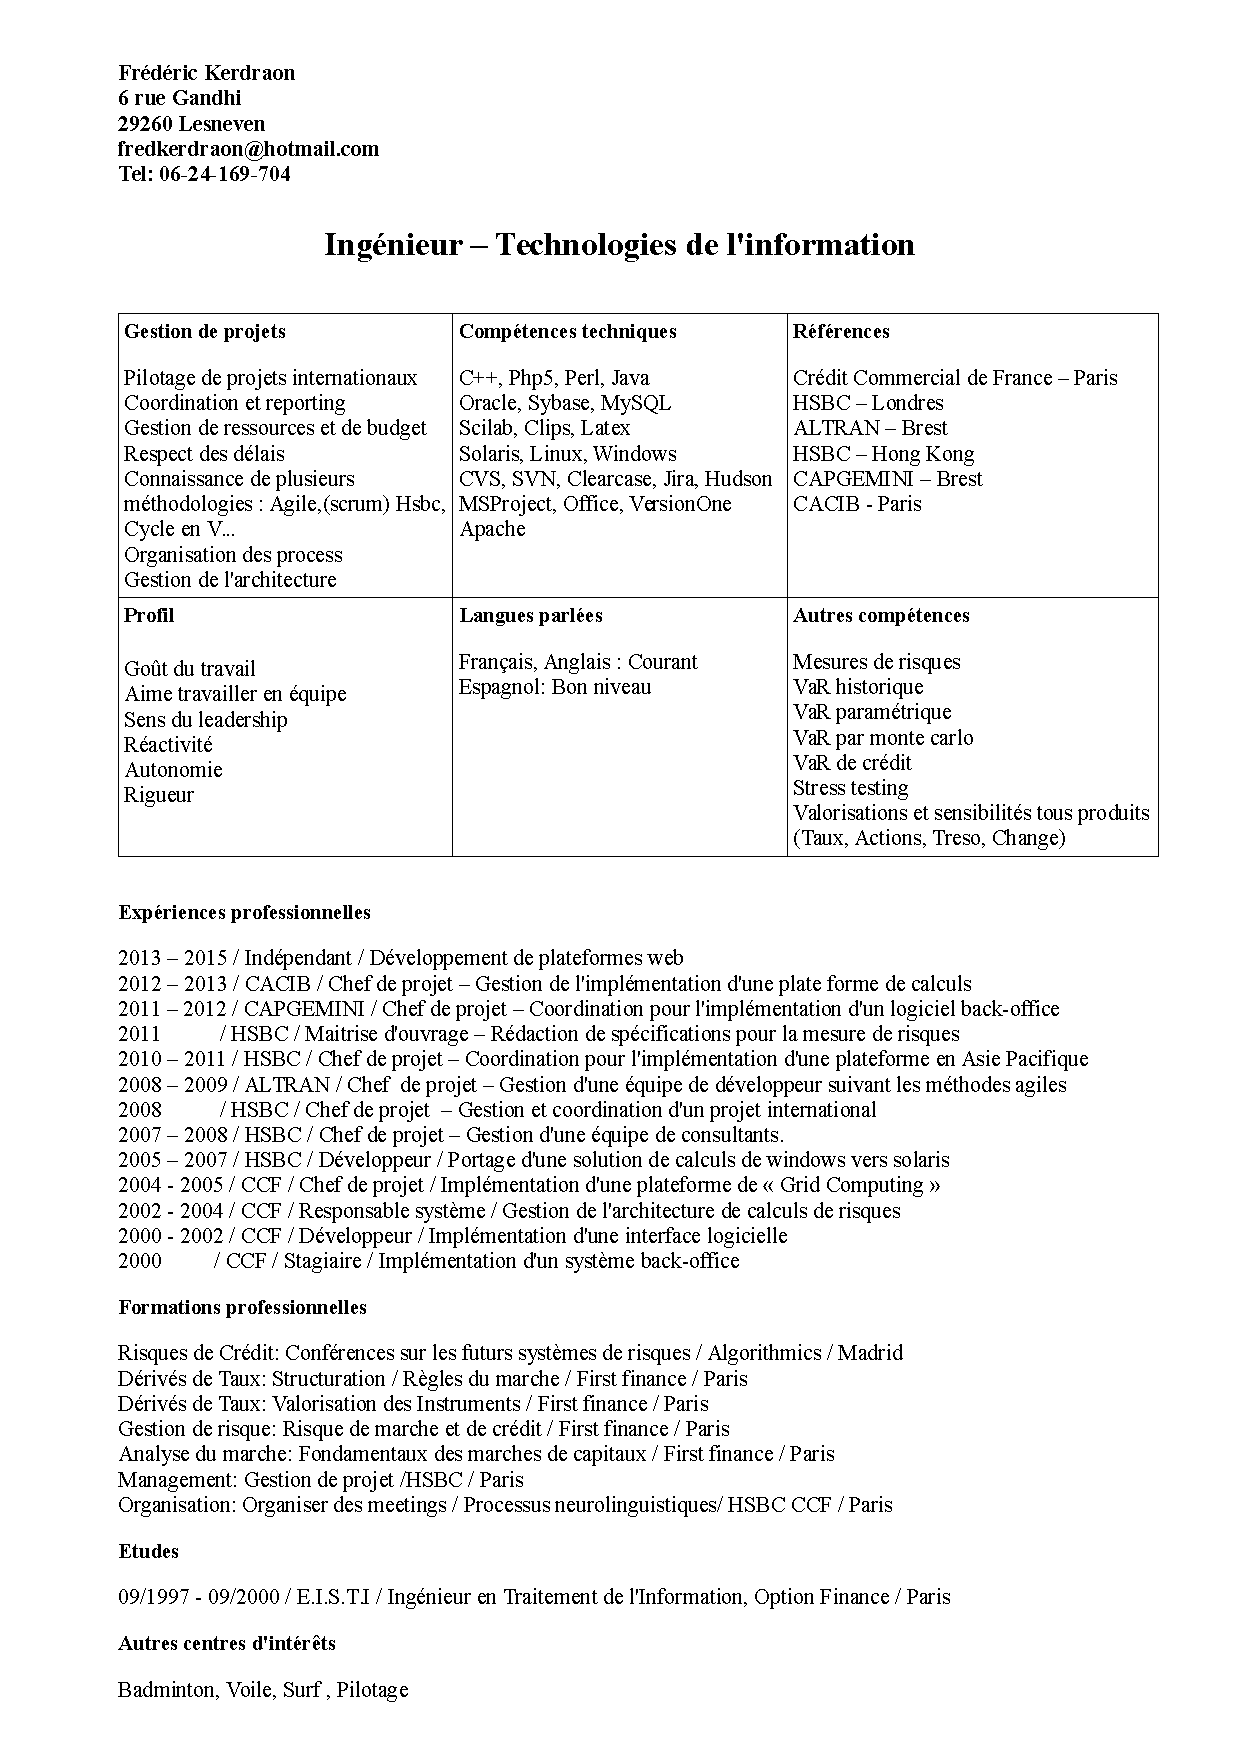
\includepdf[pages={1}]{Resume.pdf}
%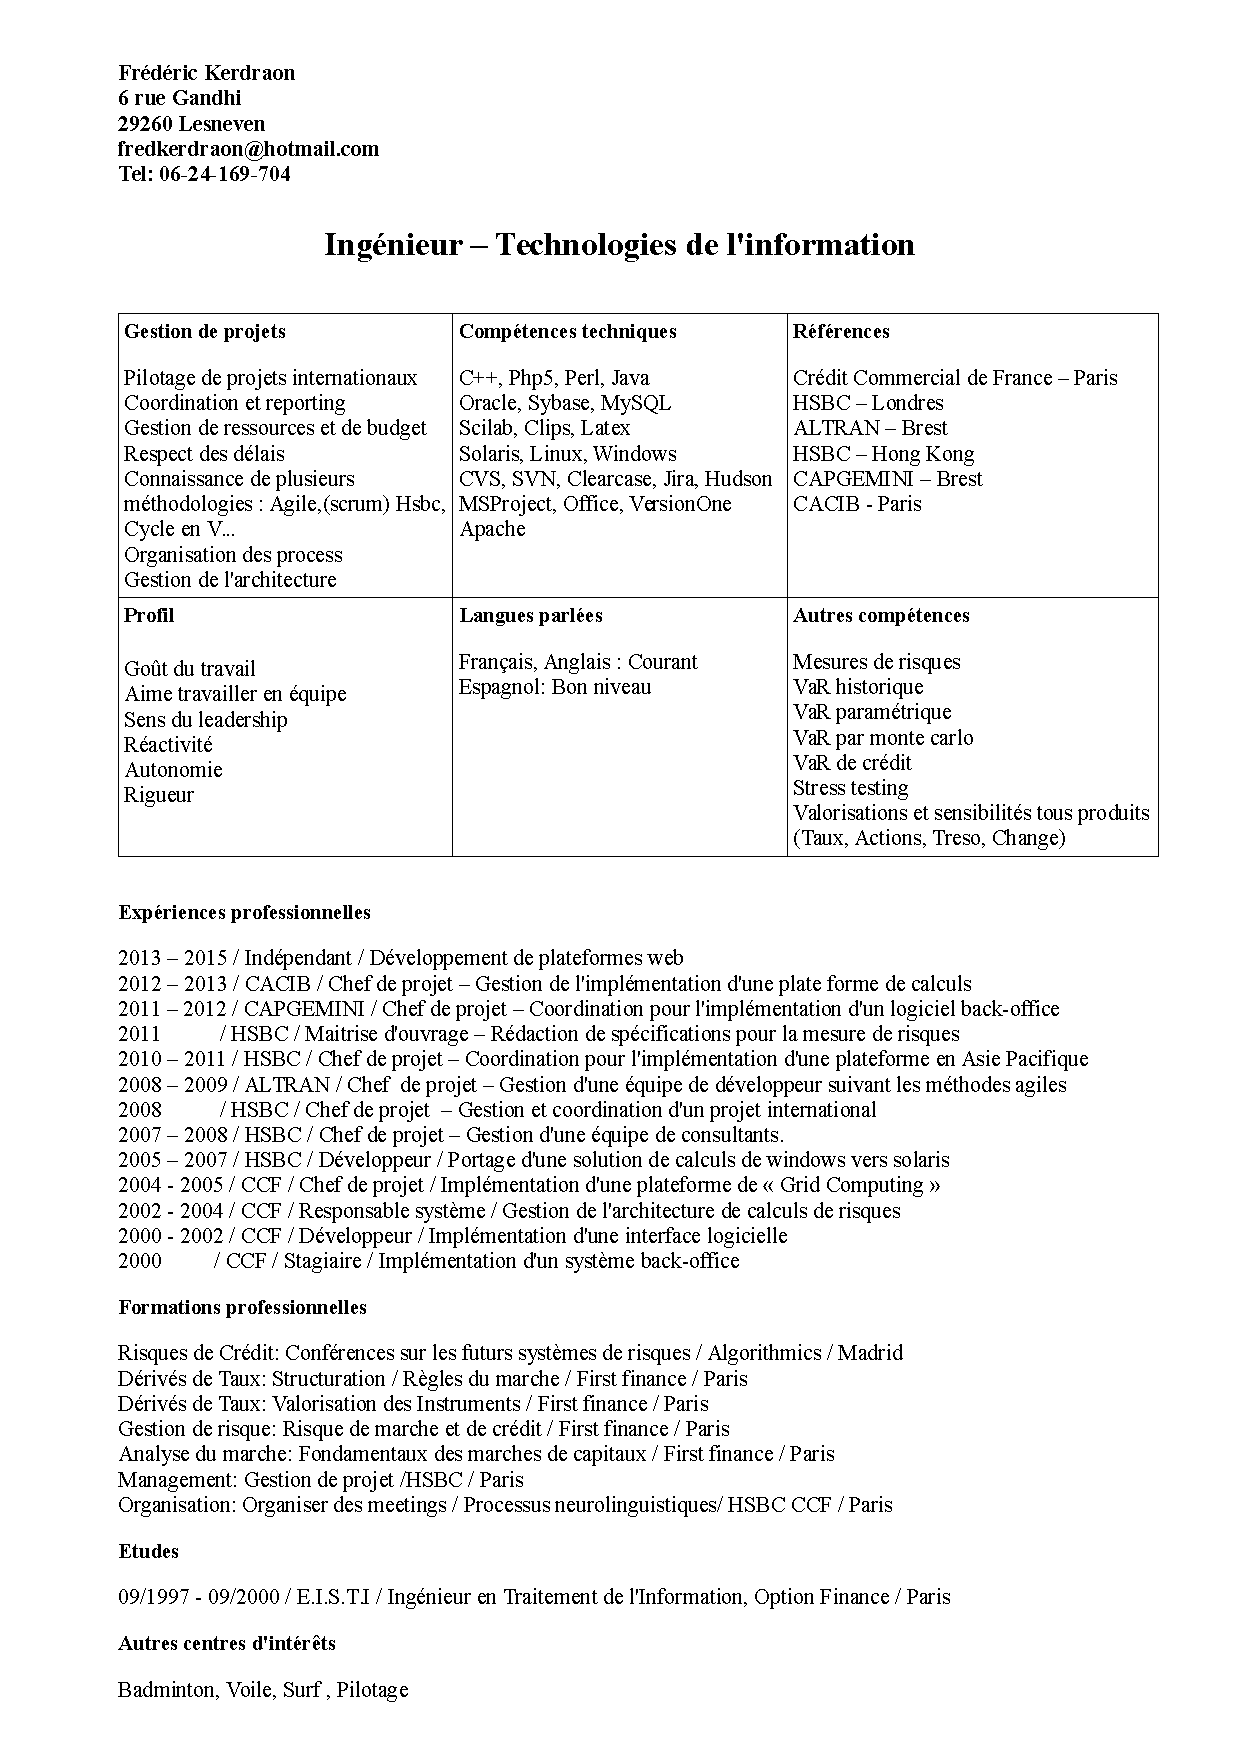
\includegraphics[width=200pts]{Resume.pdf}
%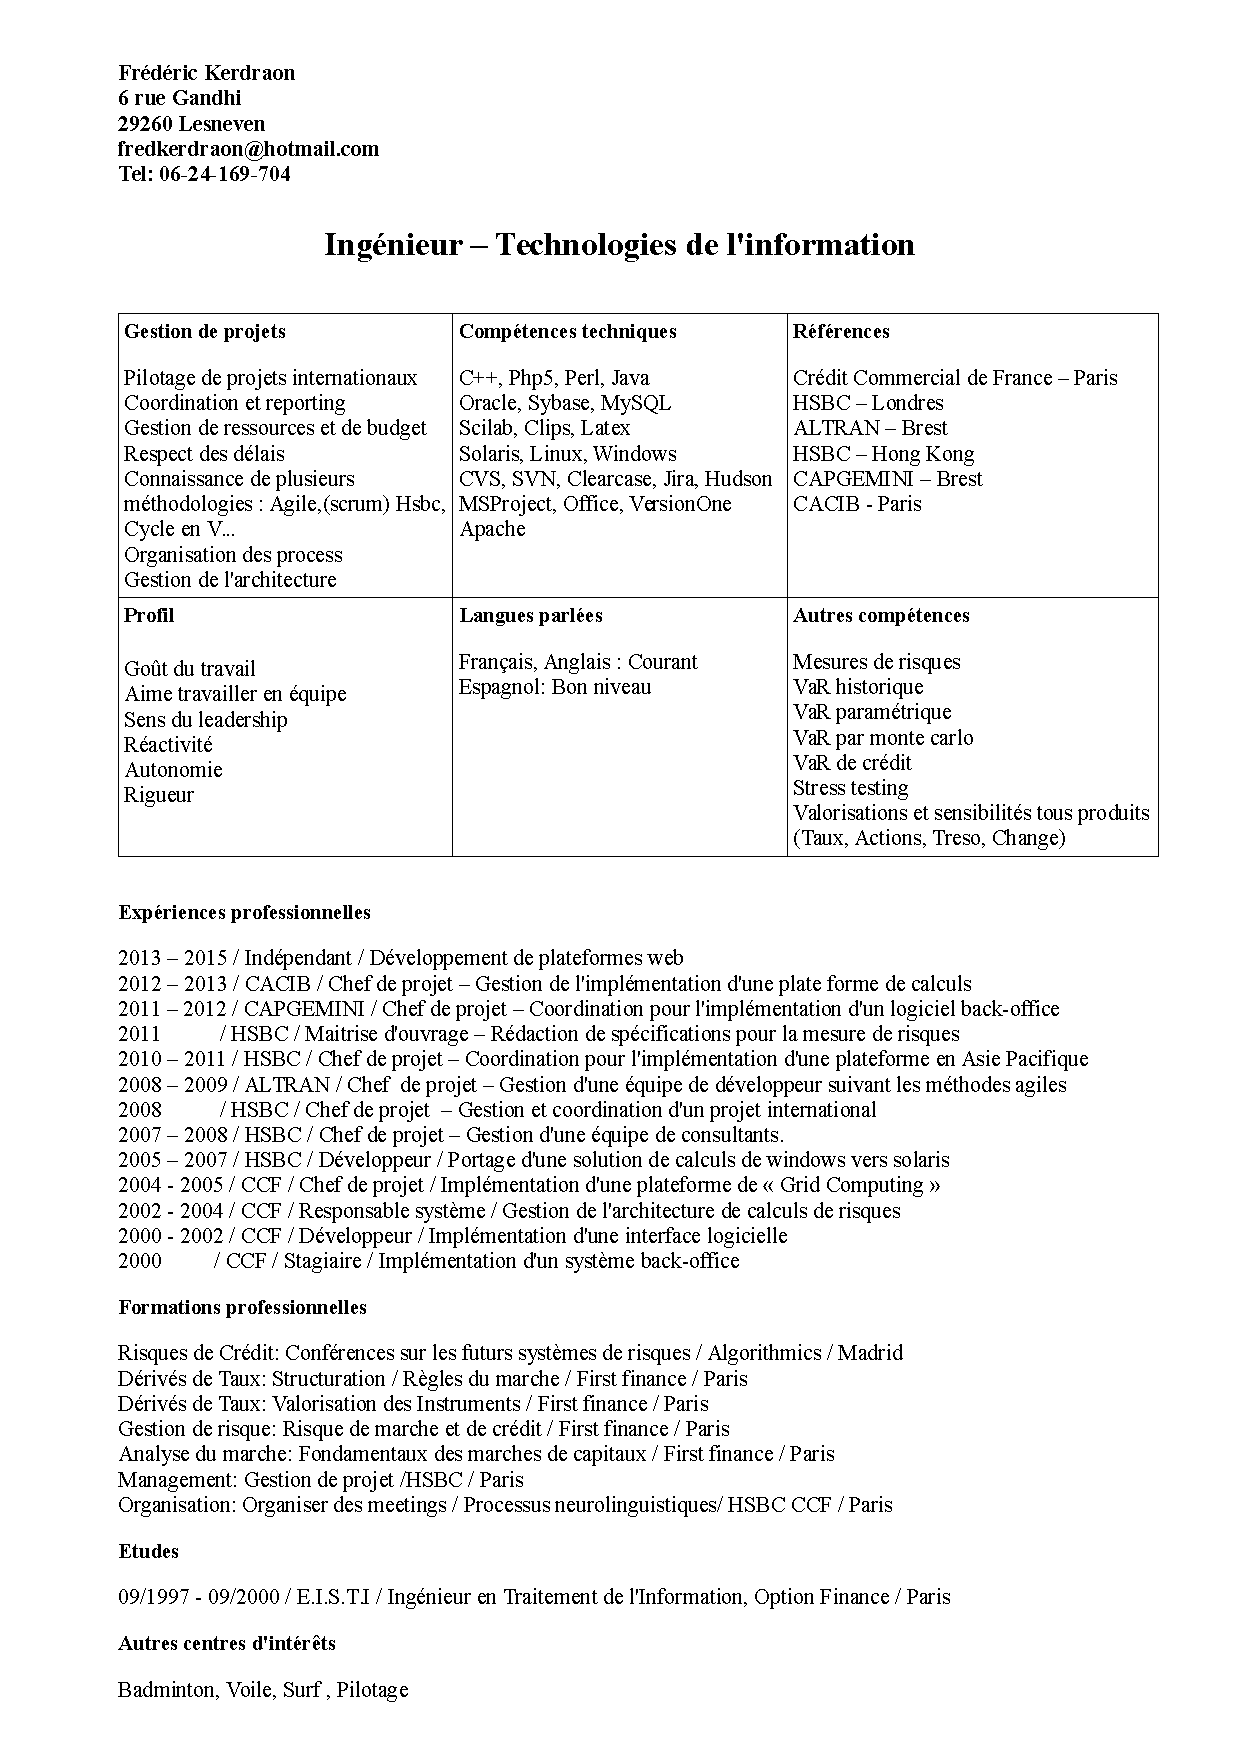
\includegraphics[scale=0.5]{Resume.pdf}}
Encule, ca marche pas!!!!
\begin{itemize}
  \item Contact1 
  \item Contact2 
  \item Contact3 
\end{itemize}

\subsection{Skills}

{\footnotesize
\subsubsection{Data}
\begin{longtable}{|c|c|c|c|c|c|}
\hline
\multicolumn{6}{|c|}{Skills} \\
\hline
ID & Contact & Name & Rating & Experience & Reference\\
\hline
23 & Fred & Football & 1000 & 0 & Louis\\
\hline
1 & Fred & Project-management & 850 & 0 & Mark\\
\hline
2 & Fred & Finance & 700 & 0 & Pete\\
\hline
3 & Fred & Risk-management & 550 & 0 & Pete\\
\hline
4 & Fred & Organisation & 400 & 0 & Phil\\
\hline
7 & Fred & Career-development & 250 & 0 & Toto\\
\hline
9 & Fred & Information-technology & 100 & 0 & Toto\\
\hline
13 & Fred & Sports & 90 & 0 & Toto\\
\hline
 ... & ... & ... & ... & ... & ... \\
\hline
 & & Total & 4502 &  & \\
\hline
\end{longtable}

\subsubsection{Graph}
\begin{bchart}[min=0,max=1000,step=200,unit=K\texteuro]
\bcbar[label=Football]{1000}\\
\smallskip
\bcbar[label=Project-management]{850}\\
\smallskip
\bcbar[label=Finance]{700}\\
\smallskip
\bcbar[label=Risk-management]{550}\\
\smallskip
\bcbar[label=Organisation]{400}\\
\smallskip
\bcbar[label=Career-development]{250}\\
\smallskip
\bcbar[label=Information-technology]{100}\\
\smallskip
\bcbar[label=Sports]{90}\\
\smallskip
\end{bchart}

\subsubsection{Cheese}
\begin{tikzpicture}[scale=1.2]
\foreach \p/\t in {
22 / Football-1000K\texteuro ,
18 / Project-management-850K\texteuro ,
15 / Finance-700K\texteuro ,
12 / Risk-management-550K\texteuro ,
8 / Organisation-400K\texteuro ,
5 / Career-development-250K\texteuro ,
2 / Information-technology-100K\texteuro ,
1 / Sports-90K\texteuro 
}
  {
\setcounter{a}{\value{b}}
\addtocounter{b}{\p}
\slice{\thea/100*360}
          {\theb/100*360}
          {\p\%}{\t}
  }
\end{tikzpicture}

}

\subsection{Acheivements}

Take a look at : http://localhost/Joomla/index.php
Ca marche les références, mais c'est pas beau!
\href{http://localhost/Joomla/index.php}{Joomla}
\begin{itemize}
  \item Contact1 
  \item Contact2 
  \item Contact3 
\end{itemize}

\subsection{Curriculum}
{\footnotesize
Will include my resume as a pdf here\\
\begin{itemize}
  \item Contact1 
  \item Contact2 
  \item Contact3 
\end{itemize}
}

\subsection{Contacts}

{\footnotesize
\subsubsection{Data}
\begin{longtable}{|c|c|c|c|c|}
\hline
\multicolumn{5}{|c|}{Contacts} \\
\hline
ID & Name & Rating & Town & Telephone\\
\hline
101 & Wing & 1000 & HongKong & 85296001395\\
\hline
108 & Zazzy & 900 & Brest & 33611037735\\
\hline
27 & Flozio & 850 & Brest & 33680938975\\
\hline
24 & Fanch & 800 & Brest & 33685769214\\
\hline
68 & Mummy & 800 & Brest & 33674340108\\
\hline
89 & Sonia & 600 & Rennes & 33612425946\\
\hline
83 & Rico & 550 & Brest & 33611037992\\
\hline
60 & Maeva & 500 & Brest & 33662575512\\
\hline
42 & Jessie & 500 & Brest & 33681775660\\
\hline
41 & Jessica & 500 & Brest & 699114929\\
\hline
23 & Etienne & 400 & Brest & 619144832\\
\hline
2 & Armelle & 400 & Brest & 33677134026\\
\hline
96 & Tiprig & 250 & Paris & 33663626188\\
\hline
22 & Elise & 250 & ???? & 33614921085\\
\hline
 ... & ... & ... & ... & ... \\
\hline
Total & 8300 &  & & \\
\hline
\end{longtable}

\subsubsection{Graph}
\begin{bchart}[min=0,max=1000,step=200,unit=K\texteuro]
\bcbar[label=Wing]{1000}\\
\smallskip
\bcbar[label=Zazzy]{900}\\
\smallskip
\bcbar[label=Flozio]{850}\\
\smallskip
\bcbar[label=Fanch]{800}\\
\smallskip
\bcbar[label=Mummy]{800}\\
\smallskip
\bcbar[label=Sonia]{600}\\
\smallskip
\bcbar[label=Rico]{550}\\
\smallskip
\bcbar[label=Maeva]{500}\\
\smallskip
\bcbar[label=Jessie]{500}\\
\smallskip
\bcbar[label=Jessica]{500}\\
\smallskip
\bcbar[label=Etienne]{400}\\
\smallskip
\bcbar[label=Armelle]{400}\\
\smallskip
\bcbar[label=Tiprig]{250}\\
\smallskip
\bcbar[label=Elise]{250}\\
\smallskip
\end{bchart}

\subsubsection{Cheese}
\begin{tikzpicture}[scale=3]
\foreach \p/\t in {
12 / Wing-1000K\texteuro ,
10 / Zazzy-900K\texteuro ,
10 / Flozio-850K\texteuro ,
9 / Fanch-800K\texteuro ,
9 / Mummy-800K\texteuro ,
7 / Sonia-600K\texteuro ,
6 / Rico-550K\texteuro ,
6 / Maeva-500K\texteuro ,
6 / Jessie-500K\texteuro ,
6 / Jessica-500K\texteuro ,
4 / Etienne-400K\texteuro ,
4 / Armelle-400K\texteuro ,
3 / Tiprig-250K\texteuro ,
3 / Elise-250K\texteuro ,
}
  {
\setcounter{a}{\value{b}}
\addtocounter{b}{\p}
\slice{\thea/100*360}
          {\theb/100*360}
          {\p\%}{\t}
  }
\end{tikzpicture}

}

\section{Annexes}

\subsection{Receipes}
\begin{itemize}
  \item Contact1 
  \item Contact2 
  \item Contact3 
\end{itemize}
http://localhost/Joomla/
\subsection{Trips}
http://localhost/Joomla/
\subsection{References}
http://localhost/Joomla/
\subsection{Checklists}			
http://localhost/Joomla/
\subsection{Stats}
http://localhost/Joomla/

\end{document}
